\chapter{De Kyoto à Osaka}
\section*{3 septembre 2015}
Plus que quelques dizaines de km entre Kyoto et Osaka, dernière étape au Japon. \newline
 Je passe par Uji, petite ville de part et d'autre d'une rivière \newline
 \newline
\centerline{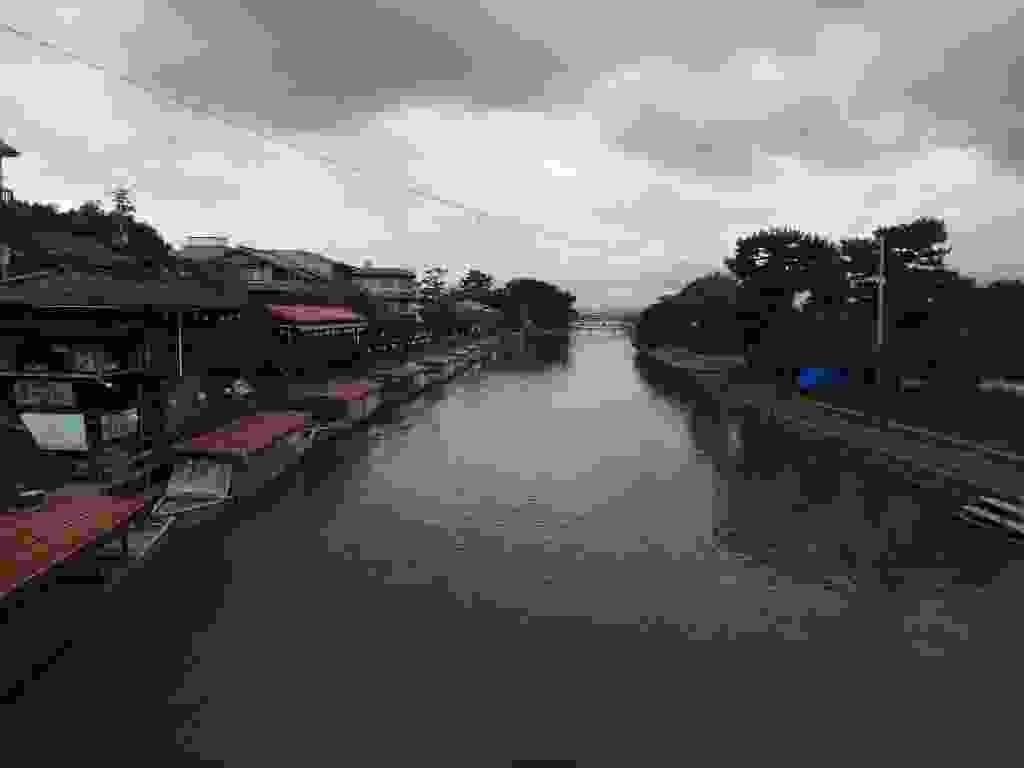
\includegraphics[width=\mywidth]{../wp-content/uploads/2015/08/P8206341-1024x768.jpg} } 
 \newline
 Le thé vert d'Uji est renommé dans tout le Japon, l'occasion d'assister à la cérémonie du thé \newline
 \newline
\centerline{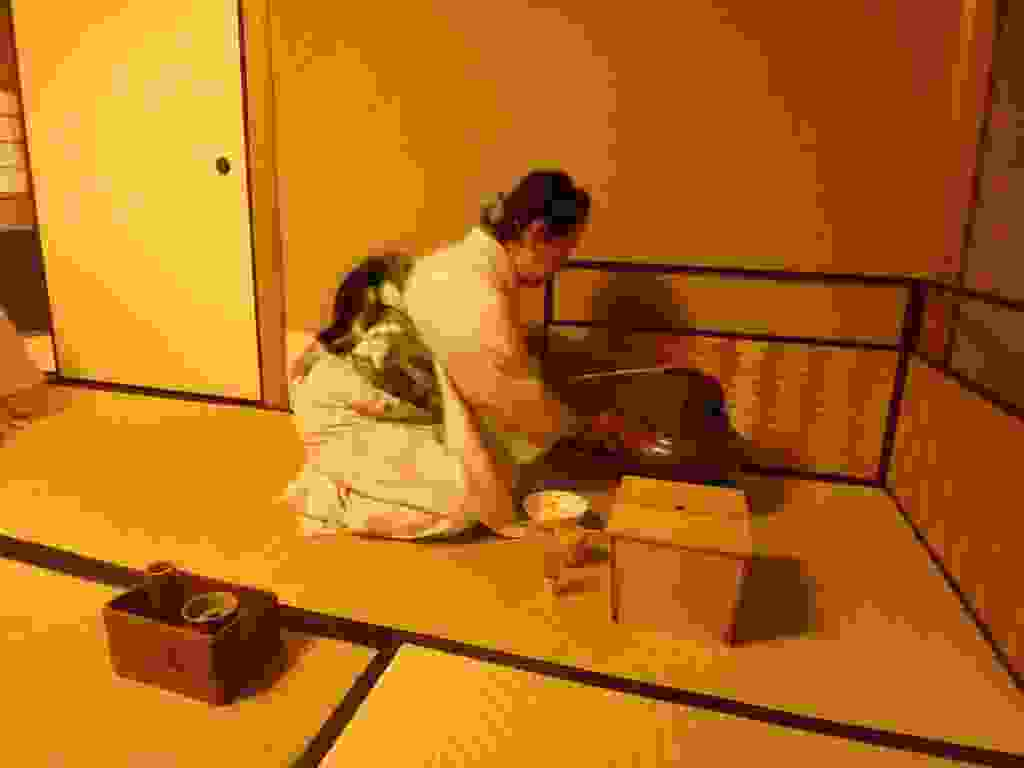
\includegraphics[width=\mywidth]{../wp-content/uploads/2015/08/P8206337-1024x768.jpg} } 
 \newline
 \newline
\centerline{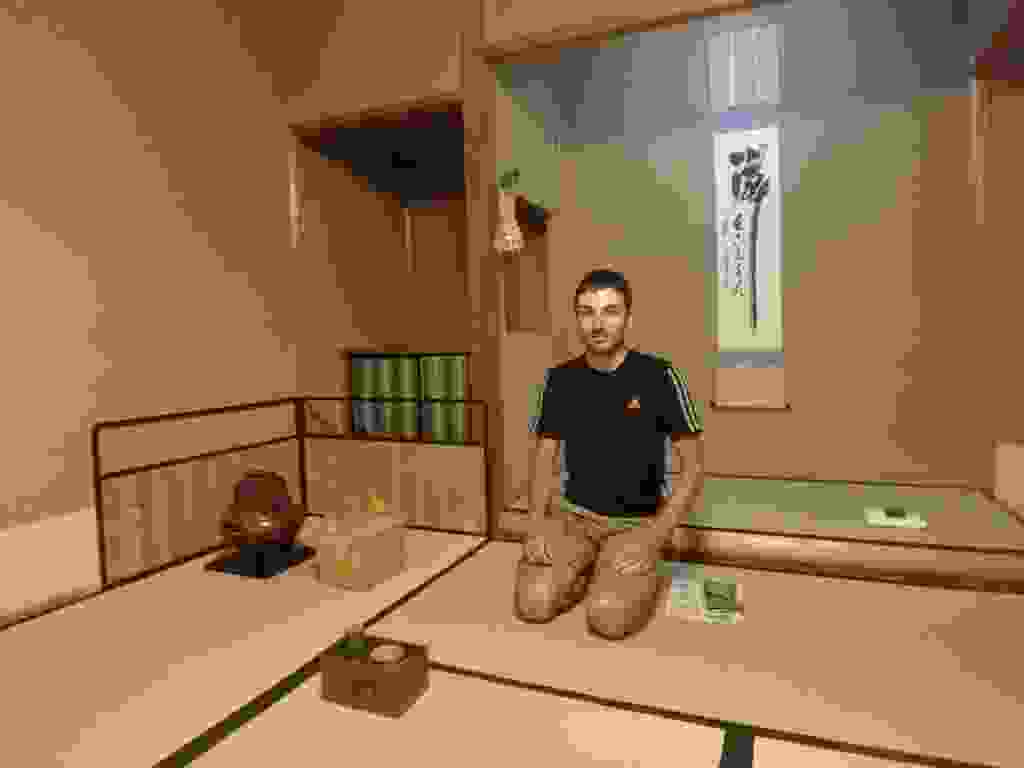
\includegraphics[width=\mywidth]{../wp-content/uploads/2015/08/P8206338-1024x768.jpg} } 
 \newline
 Deux sites intéressants à Uji : le shrine Ujigami \newline
 \newline
\centerline{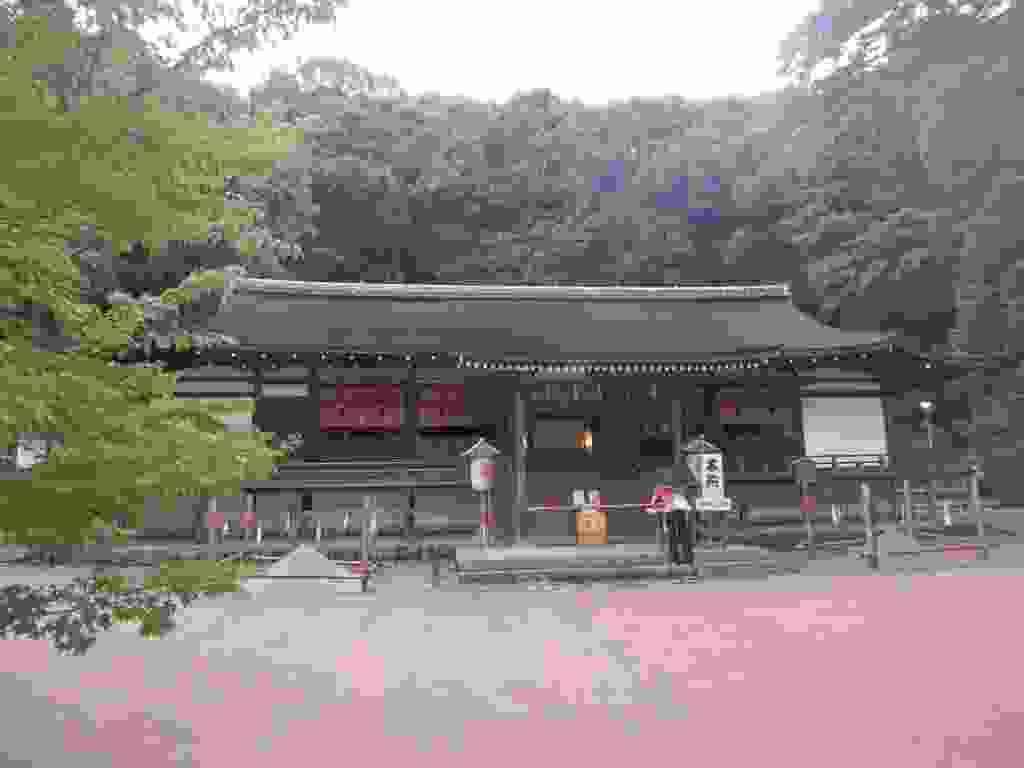
\includegraphics[width=\mywidth]{../wp-content/uploads/2015/08/P8206346-1024x768.jpg} } 
 \newline
 \newline
\centerline{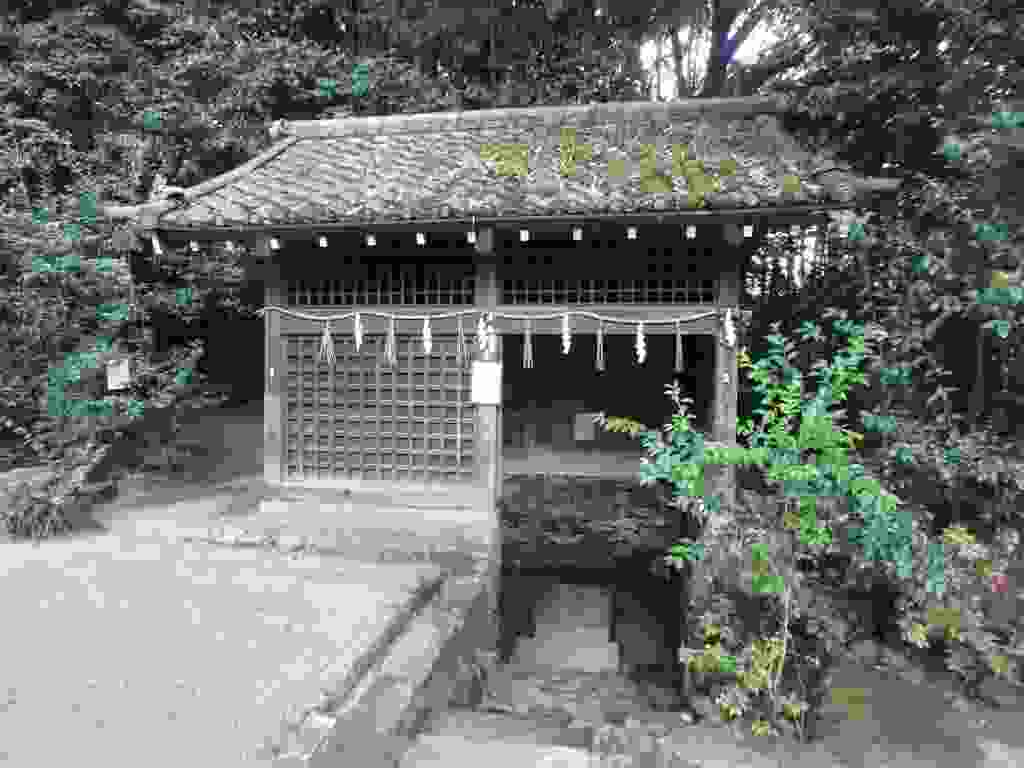
\includegraphics[width=\mywidth]{../wp-content/uploads/2015/08/P8206348-1024x768.jpg} } 
 \newline
 Et le temple Byōdō-in \newline
 \newline
\centerline{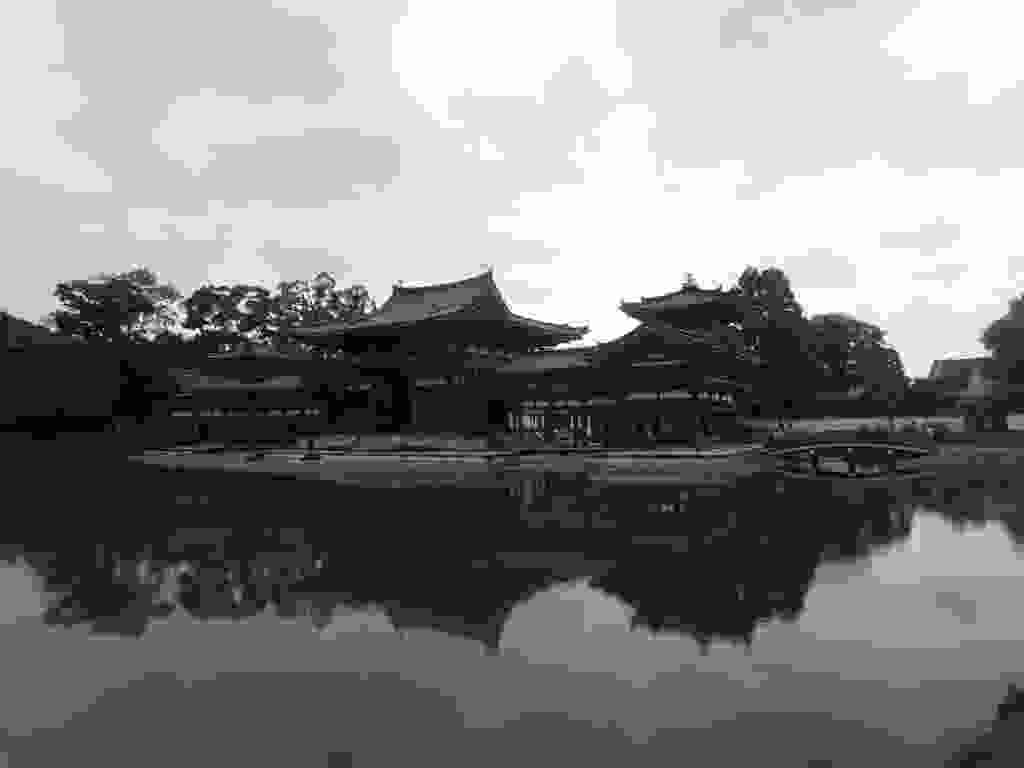
\includegraphics[width=\mywidth]{../wp-content/uploads/2015/08/P8206353-1024x768.jpg} } 
 \newline
 \newline
\centerline{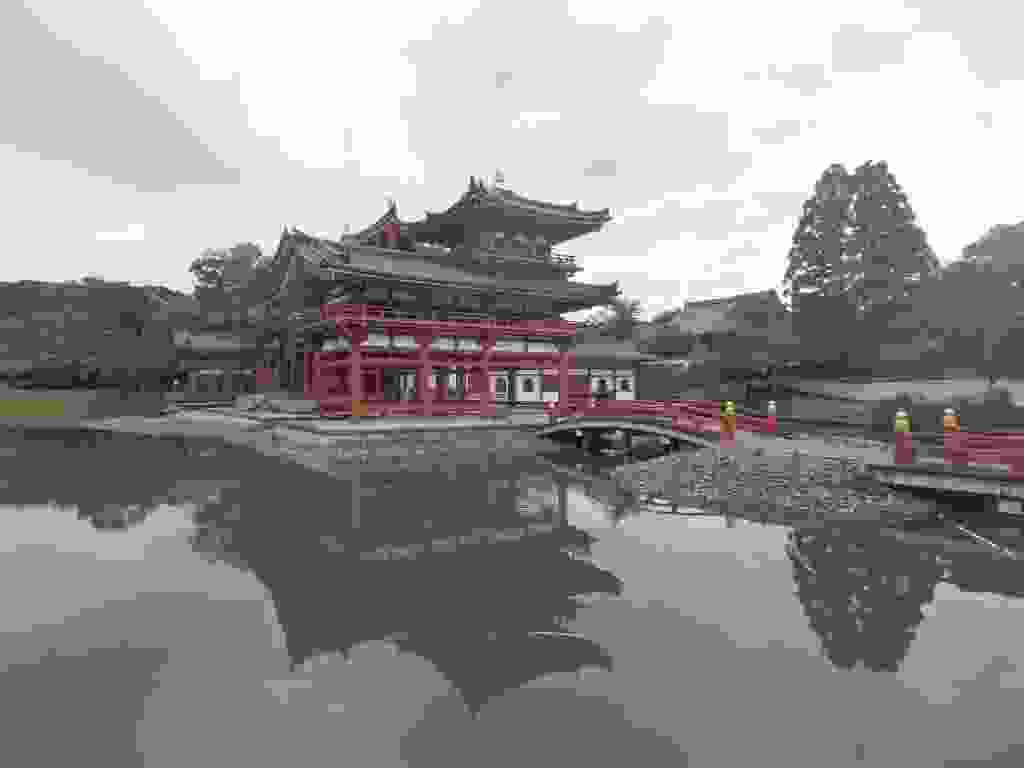
\includegraphics[width=\mywidth]{../wp-content/uploads/2015/08/P8206351-1024x768.jpg} } 
 \newline
 Je continue vers Nara, ancienne capitale du Japon. Sur la route, quelques champs de thé. \newline
 \newline
\centerline{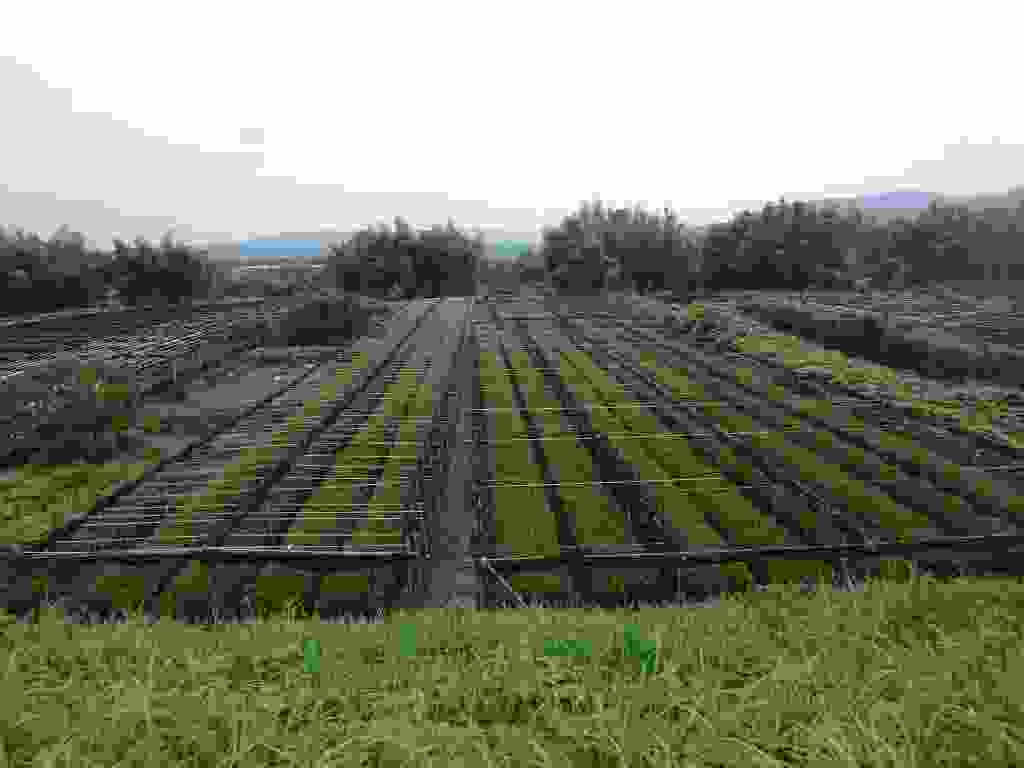
\includegraphics[width=\mywidth]{../wp-content/uploads/2015/08/P8206359-1024x768.jpg} } 
 \newline
 Parc de Nara où des centaines de cerfs pas farouches se promènent \newline
 \newline
\centerline{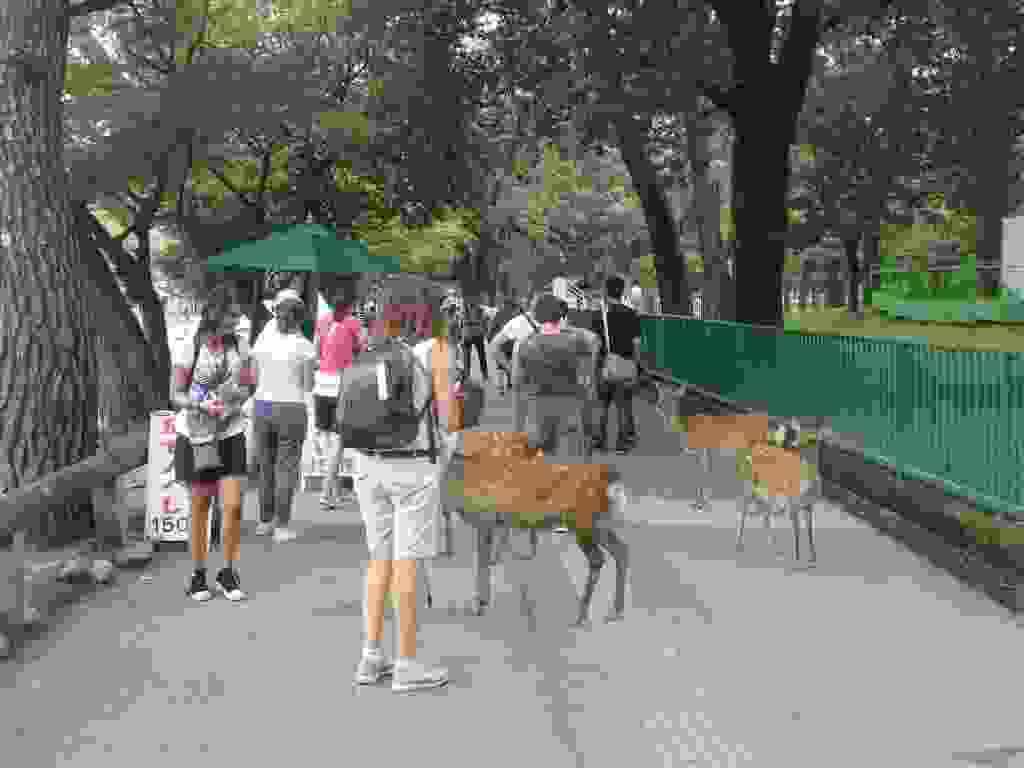
\includegraphics[width=\mywidth]{../wp-content/uploads/2015/08/P8216363-1024x768.jpg} } 
 \newline
 Joli petit jardin. En Amérique du Sud beaucoup de sites touristiques étaient plus chers pour les étrangers, ici le jardin était gratuit sauf pour les japonais. \newline
 \newline
\centerline{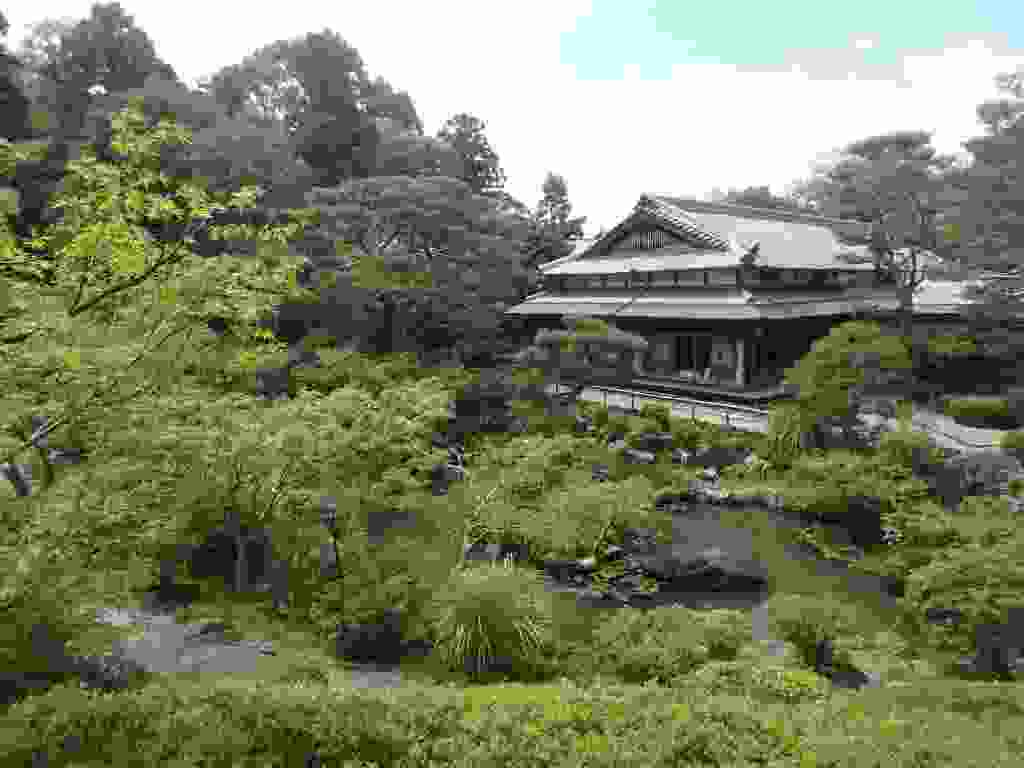
\includegraphics[width=\mywidth]{../wp-content/uploads/2015/08/P8216373-1024x768.jpg} } 
 \newline
 Le temple Tōdai-ji et son grand Buddha. Devant le temple je rencontre un cycliste allemand qui vient de faire Allemagne-Japon en 6 mois, il me dit que le pire pays qu'il a traversé est la Chine. P Parfait c'est ma prochaine destination ! \newline
 \newline
\centerline{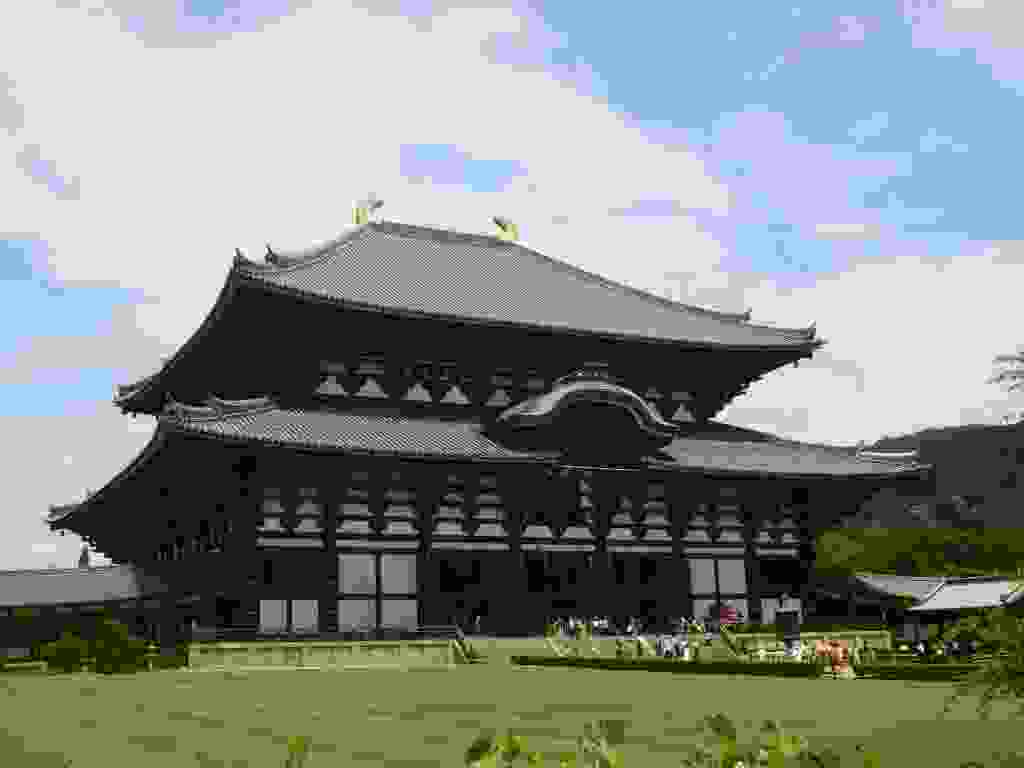
\includegraphics[width=\mywidth]{../wp-content/uploads/2015/08/P8216381-1024x768.jpg} } 
 \newline
 \newline
\centerline{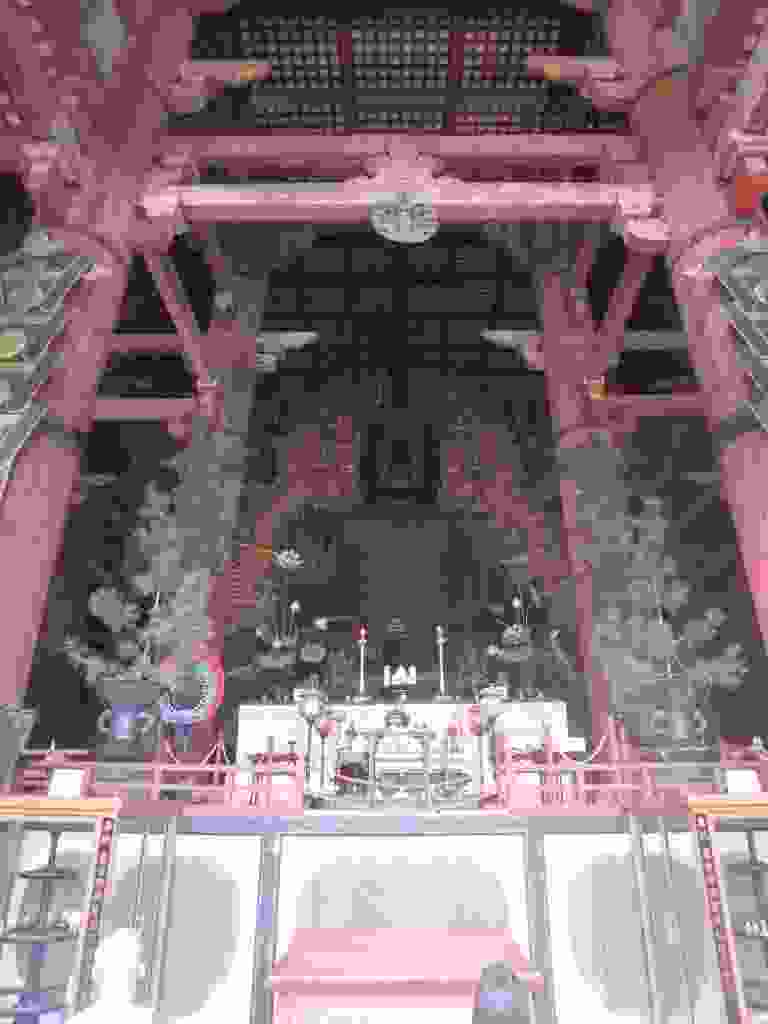
\includegraphics[width=\mywidth]{../wp-content/uploads/2015/08/P8216386-e1441019842346-768x1024.jpg} } 
 \newline
 \newline
\centerline{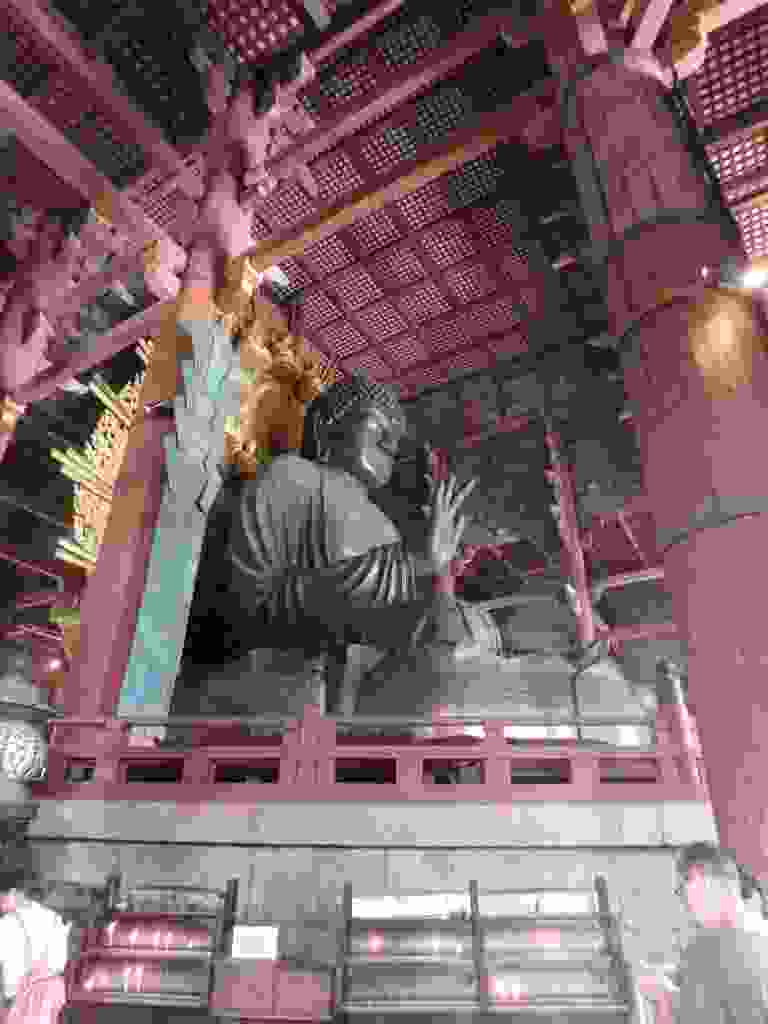
\includegraphics[width=\mywidth]{../wp-content/uploads/2015/08/P8216392-e1441029428495-768x1024.jpg} } 
 \newline
 \newline
\centerline{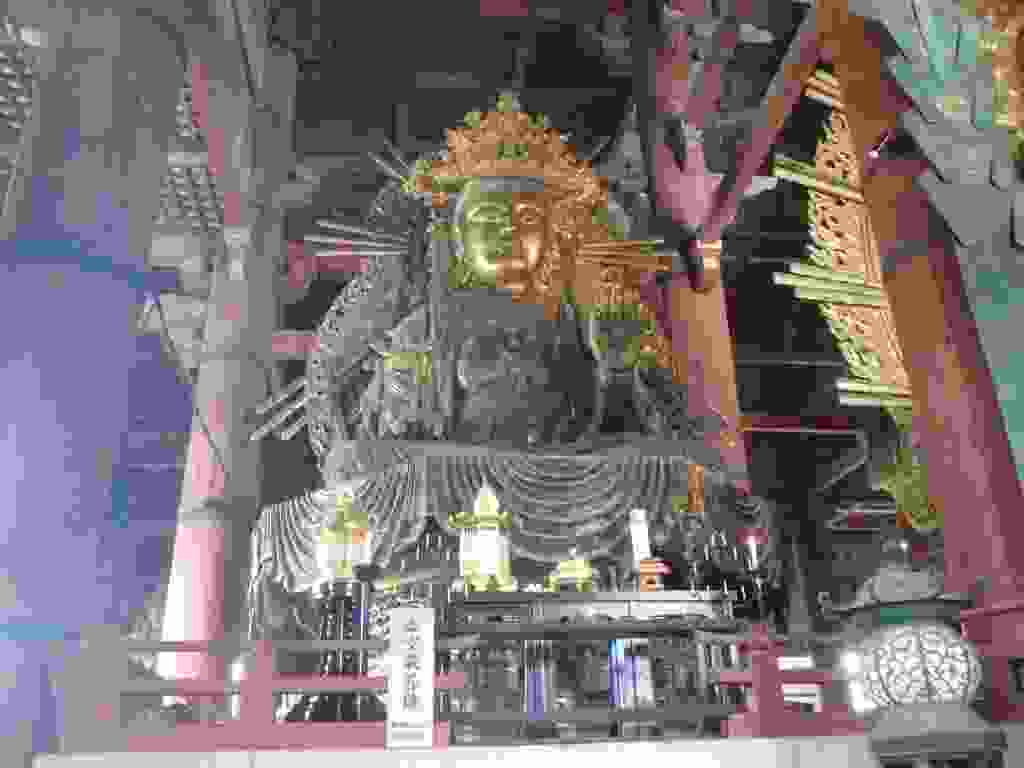
\includegraphics[width=\mywidth]{../wp-content/uploads/2015/08/P8216391-1024x768.jpg} } 
 \newline
 Le shrine Kasuga auquel on accède par un chemin bordé de milliers de lanternes \newline
 \newline
\centerline{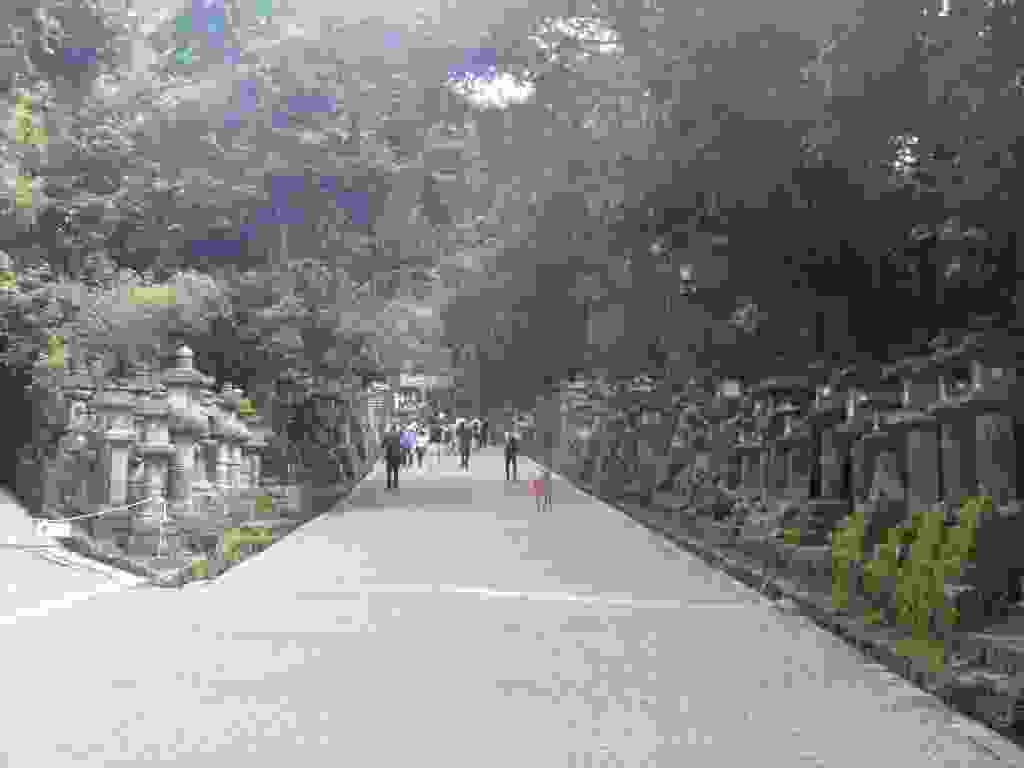
\includegraphics[width=\mywidth]{../wp-content/uploads/2015/08/P8216399-1024x768.jpg} } 
 \newline
 \newline
\centerline{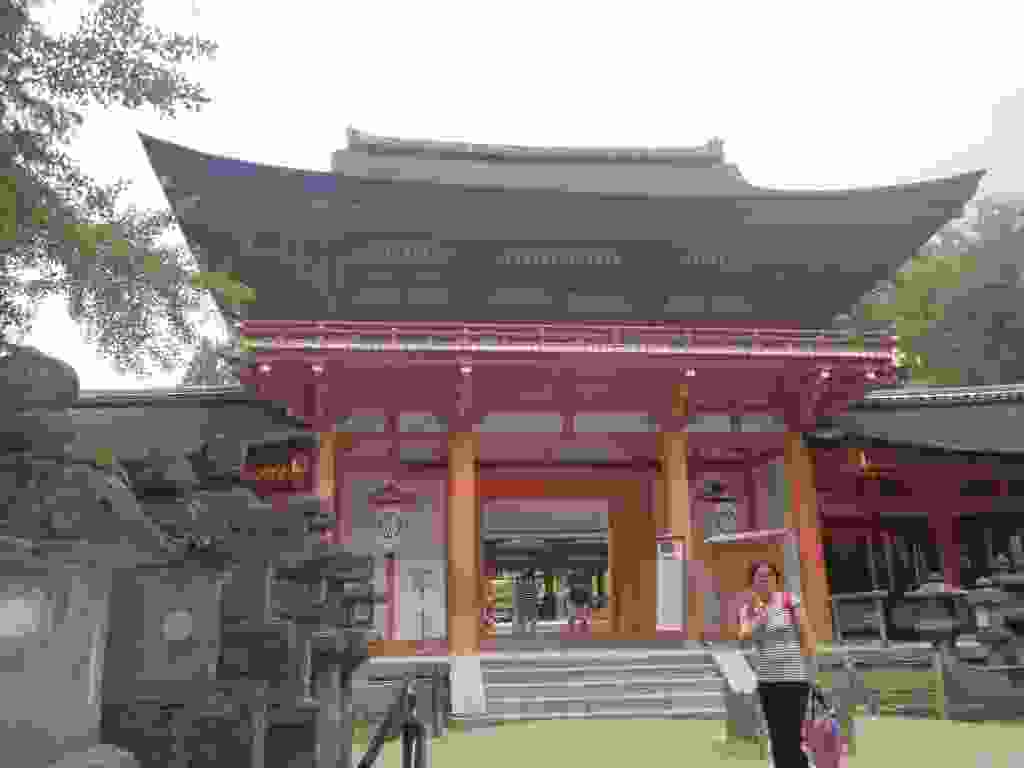
\includegraphics[width=\mywidth]{../wp-content/uploads/2015/08/P8216400-1024x768.jpg} } 
 \newline
 Comme il me reste du temps je continue jusqu'à Kobé un peu au nord d'Osaka. \newline
 Baignade rafraîchissante à la plage de Suma \newline
 \newline
\centerline{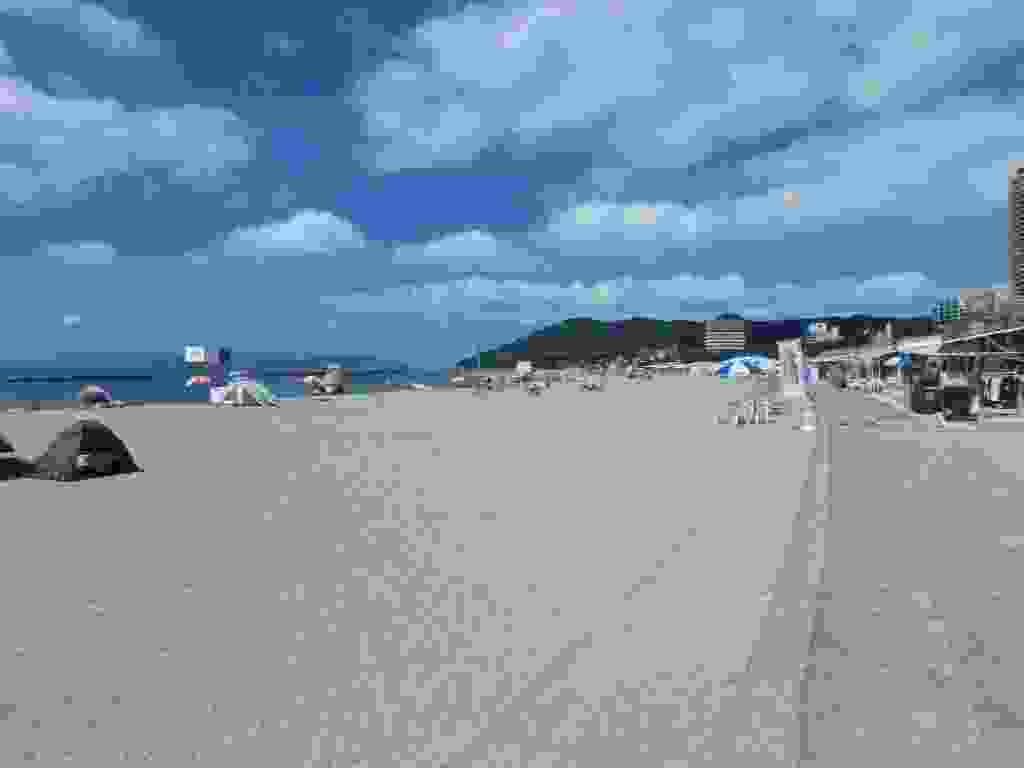
\includegraphics[width=\mywidth]{../wp-content/uploads/2015/08/P8236421-1024x768.jpg} } 
 \newline
 Quartier Sannomiya au centre de Kobé \newline
 \newline
\centerline{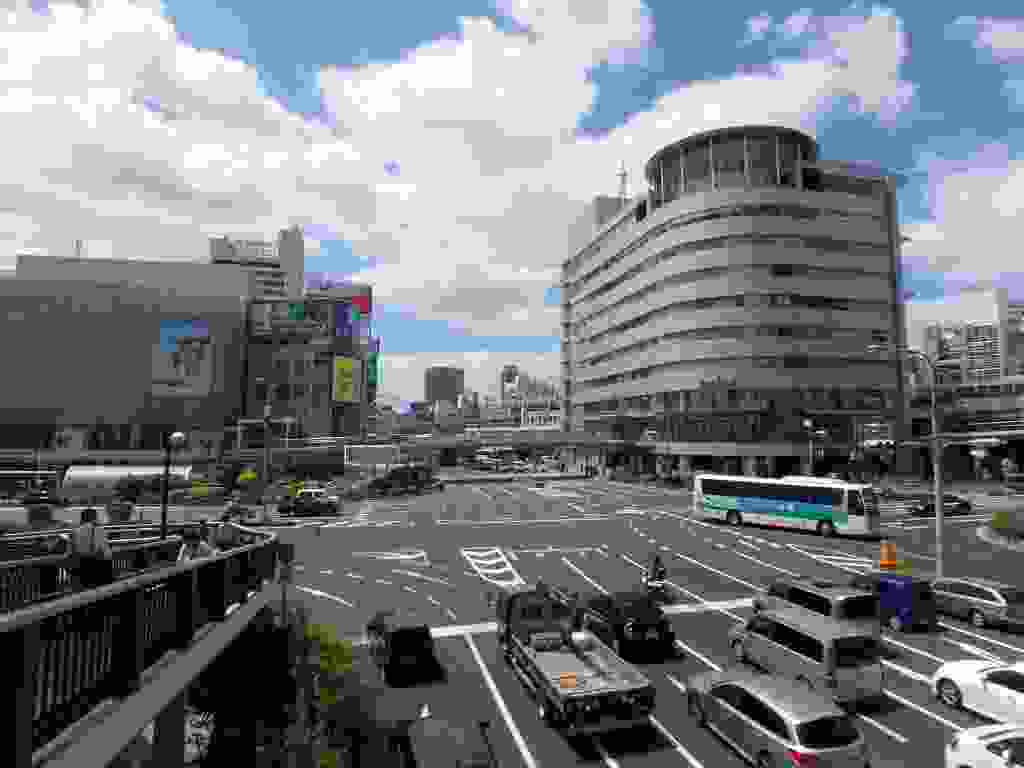
\includegraphics[width=\mywidth]{../wp-content/uploads/2015/08/P8236424-1024x768.jpg} } 
 \newline
 Influence européenne avec quelques maisons typiques \newline
 \newline
\centerline{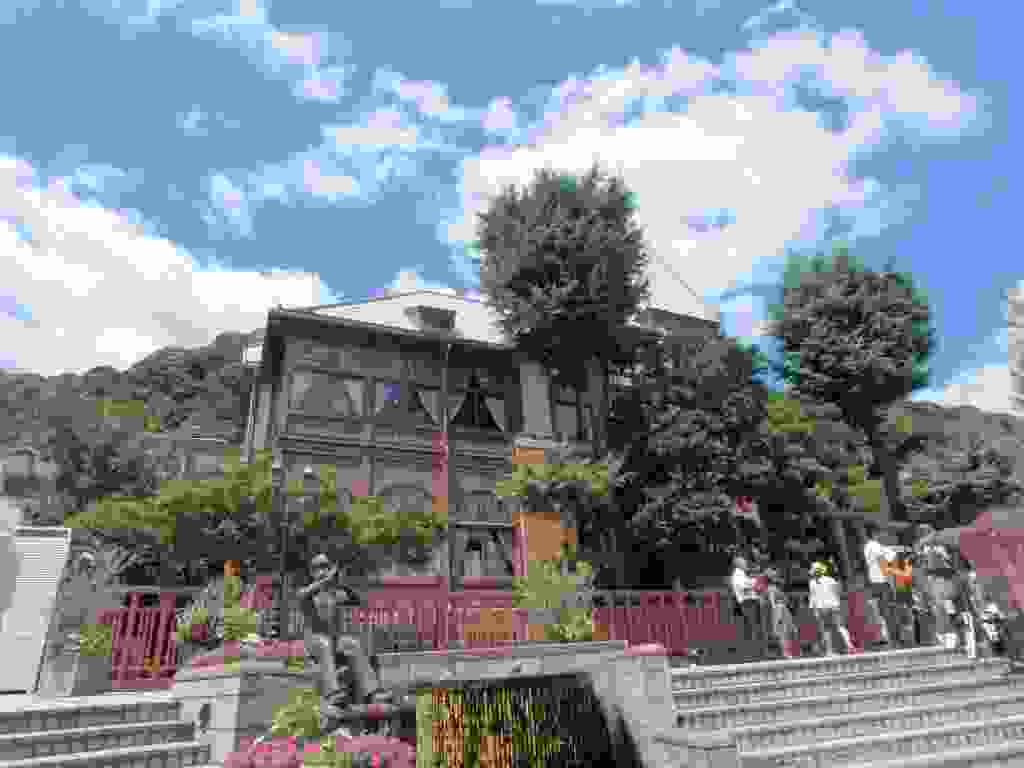
\includegraphics[width=\mywidth]{../wp-content/uploads/2015/08/P8236426-1024x768.jpg} } 
 \newline
 Le port de Kobé reconstruit après le tremblement de terre de 1995 \newline
 \newline
\centerline{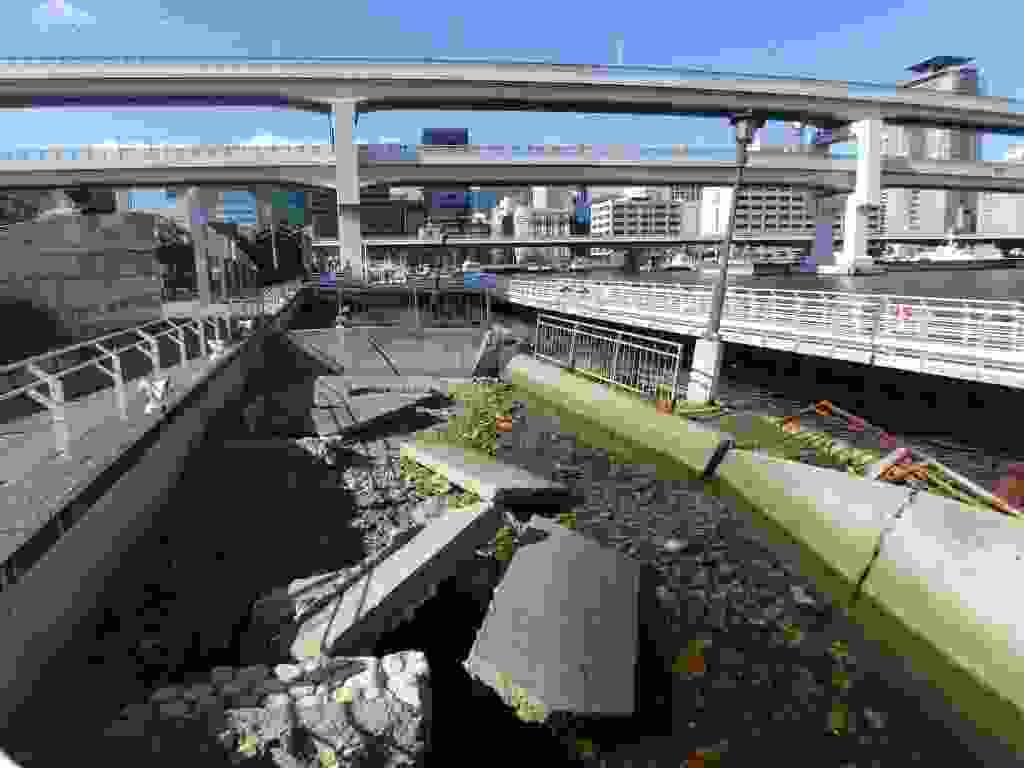
\includegraphics[width=\mywidth]{../wp-content/uploads/2015/08/P8236444-1024x768.jpg} } 
 \newline
 \newline
\centerline{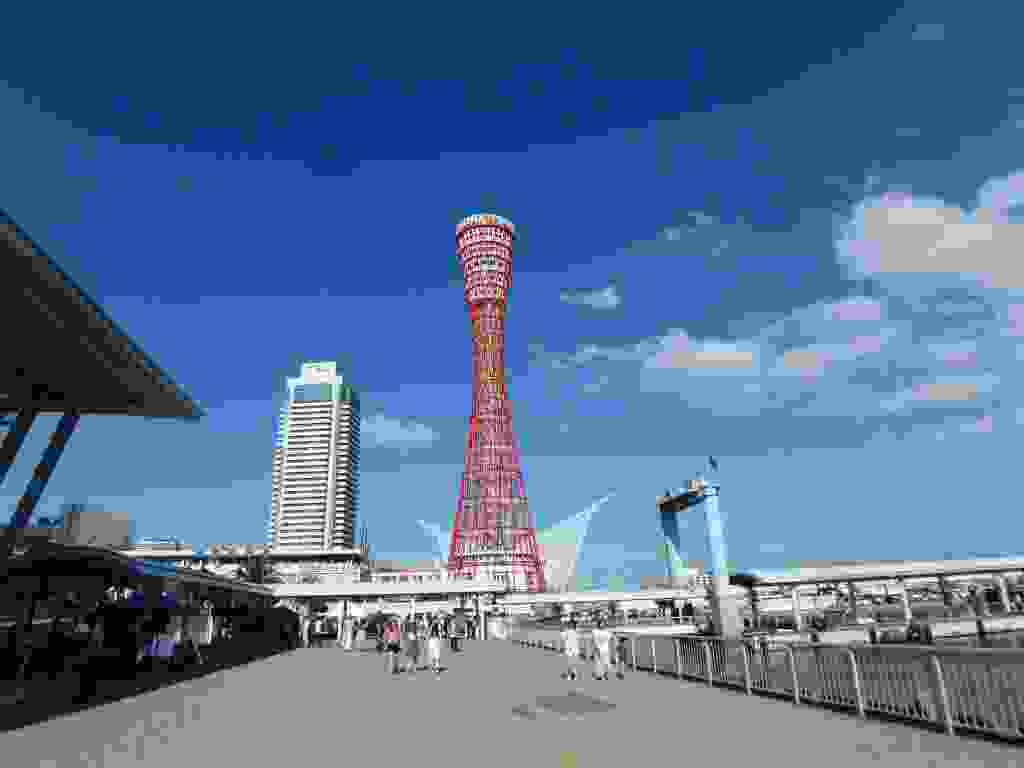
\includegraphics[width=\mywidth]{../wp-content/uploads/2015/08/P8236447-1024x768.jpg} } 
 \newline
 Visite et dégustation dans une brasserie de saké \newline
 \newline
\centerline{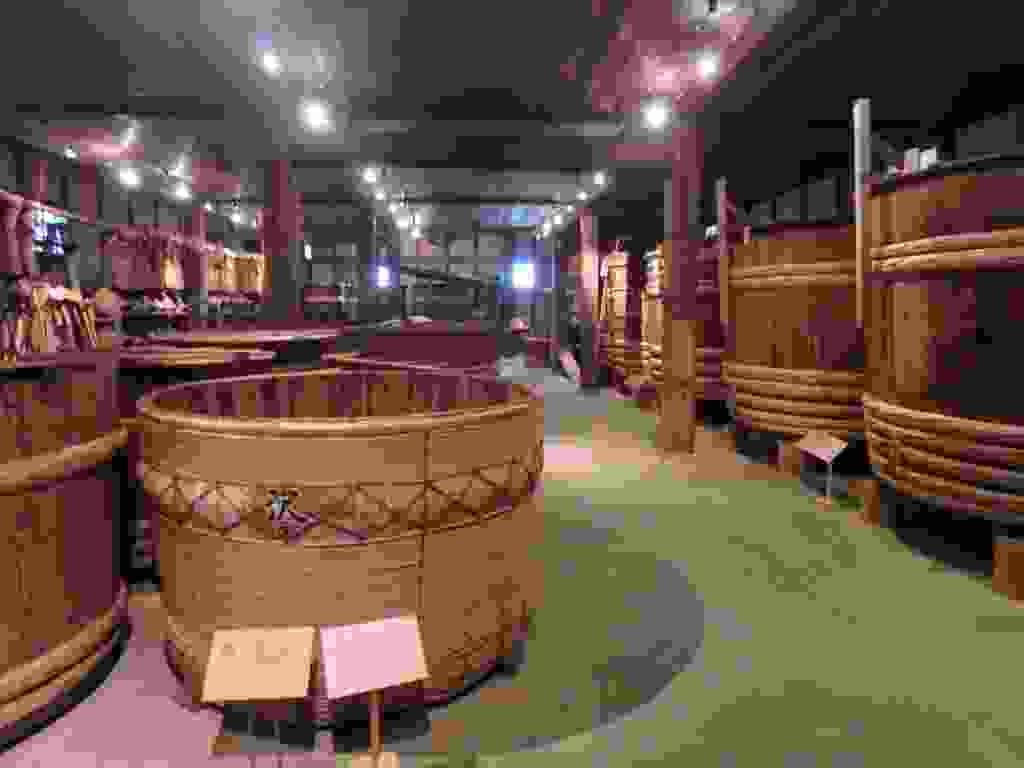
\includegraphics[width=\mywidth]{../wp-content/uploads/2015/08/P8236434-1024x768.jpg} } 
 \newline
 \newline
\centerline{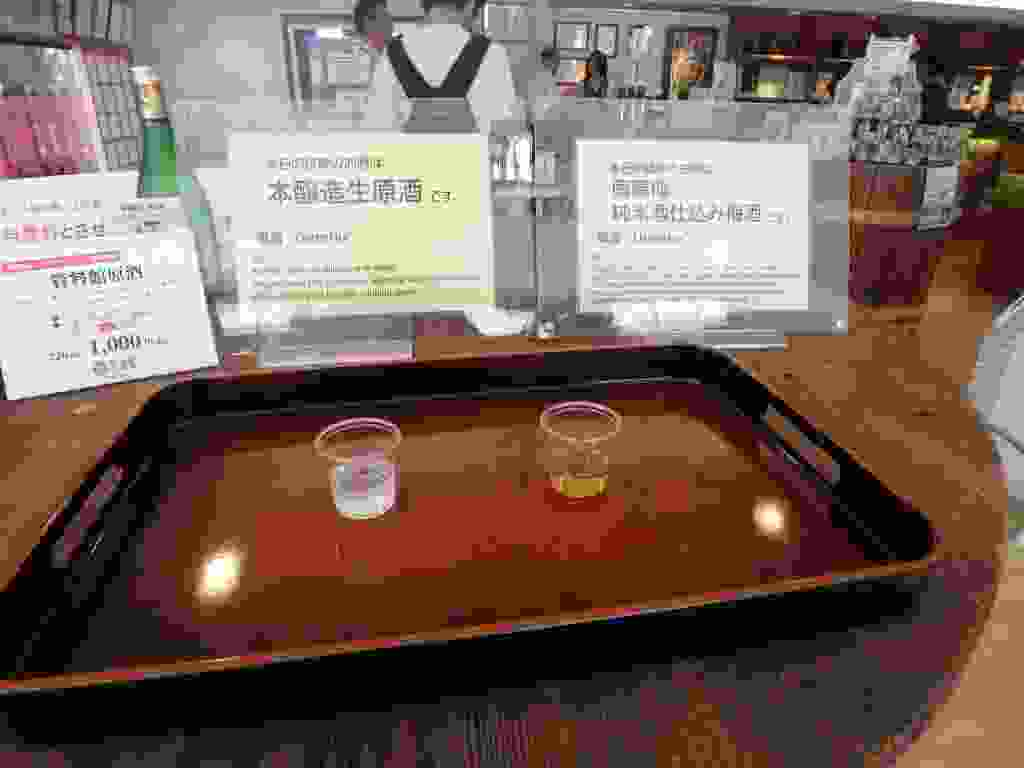
\includegraphics[width=\mywidth]{../wp-content/uploads/2015/08/P8236437-1024x768.jpg} } 
 \newline
 Pour revenir à Osaka, je fais un detour par Arima où se trouve un onsen connu \newline
 \newline
\centerline{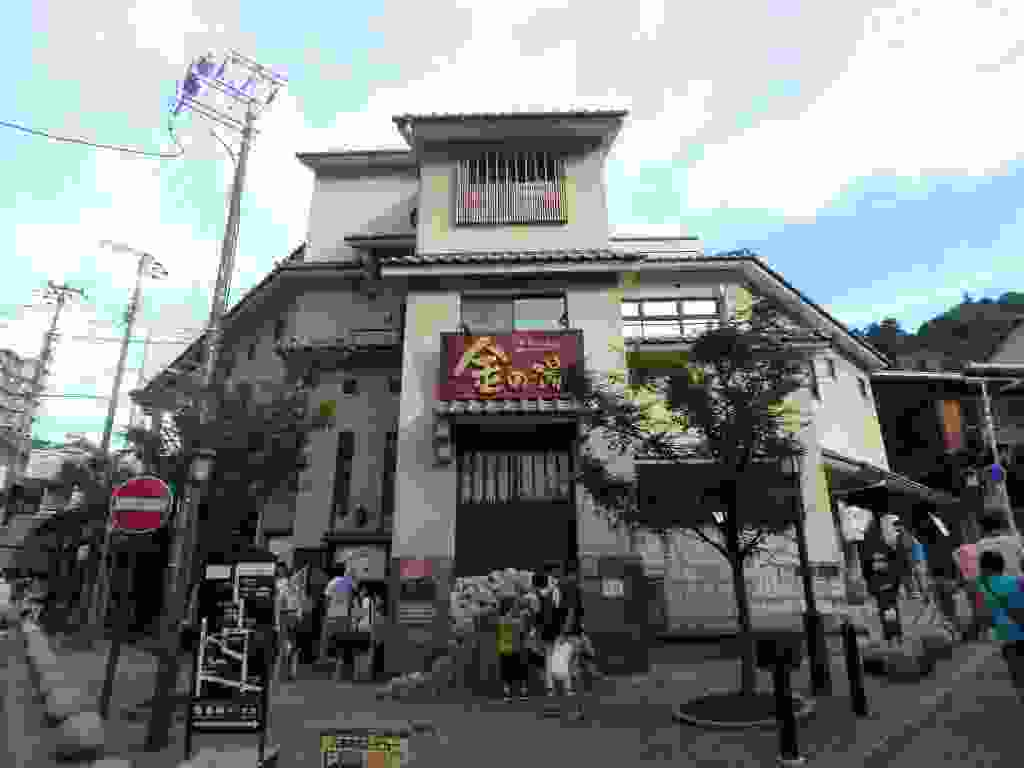
\includegraphics[width=\mywidth]{../wp-content/uploads/2015/08/P8246474-1024x768.jpg} } 
 \newline
 Depuis Arima j'accède en téléphérique au Mont Rokko à un peu plus de 900m \newline
 \newline
\centerline{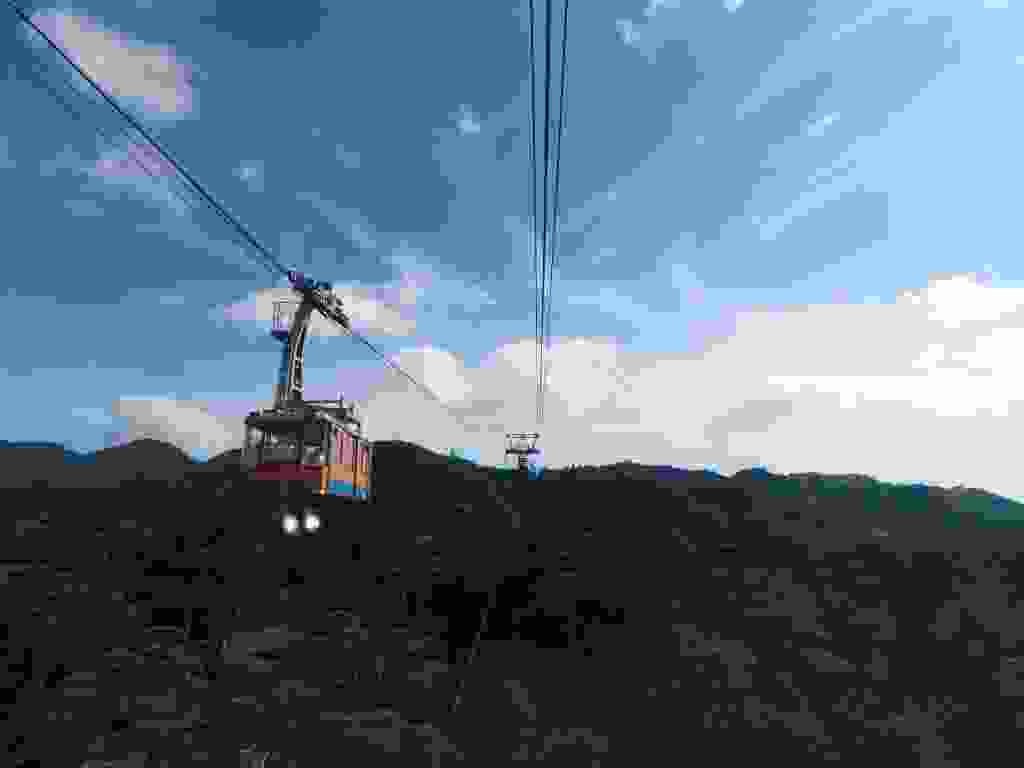
\includegraphics[width=\mywidth]{../wp-content/uploads/2015/08/P8246453-1024x768.jpg} } 
 \newline
 Belle vue sur la baie d'Osaka \newline
 \newline
\centerline{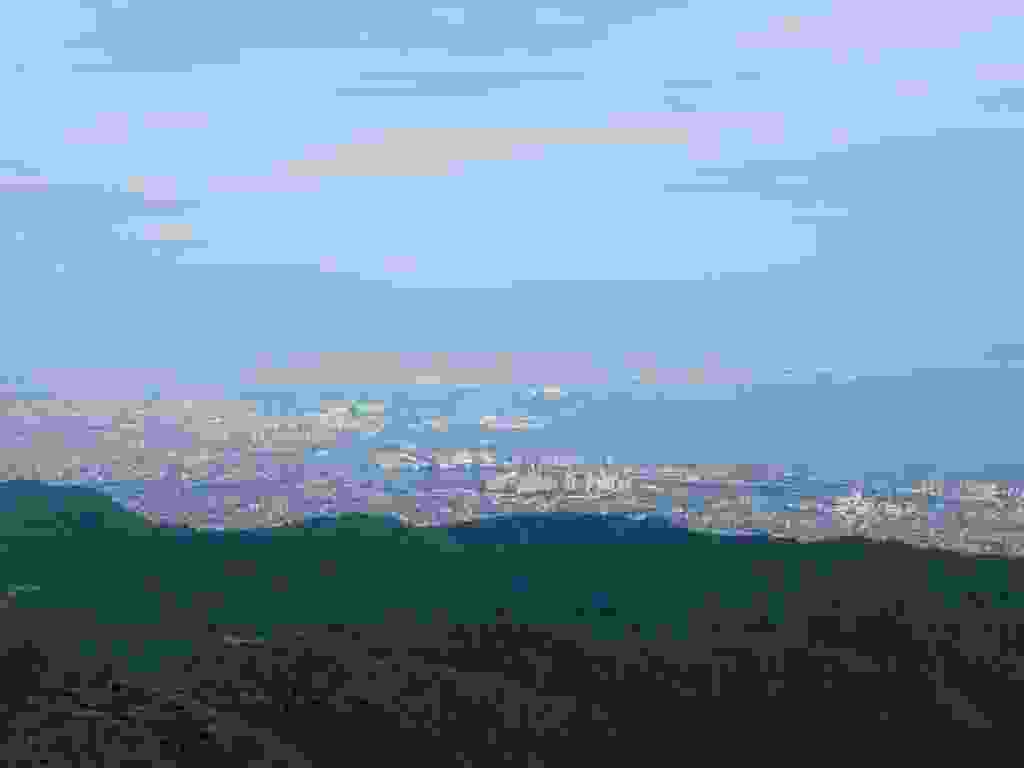
\includegraphics[width=\mywidth]{../wp-content/uploads/2015/08/P8246467-1024x768.jpg} } 
 \newline
 Osaka est presque aussi immense que Tokyo, réputée surtout pour la gastronomie et le shopping. \newline
 \newline
\centerline{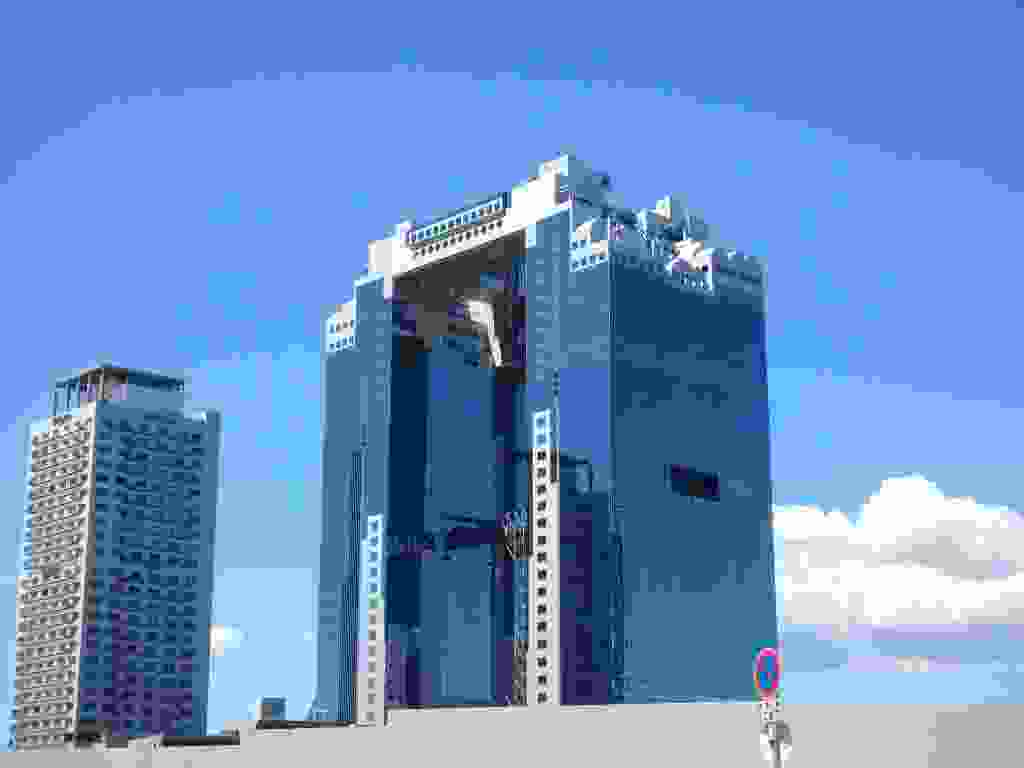
\includegraphics[width=\mywidth]{../wp-content/uploads/2015/08/P8266493-1024x768.jpg} } 
 \newline
 \newline
\centerline{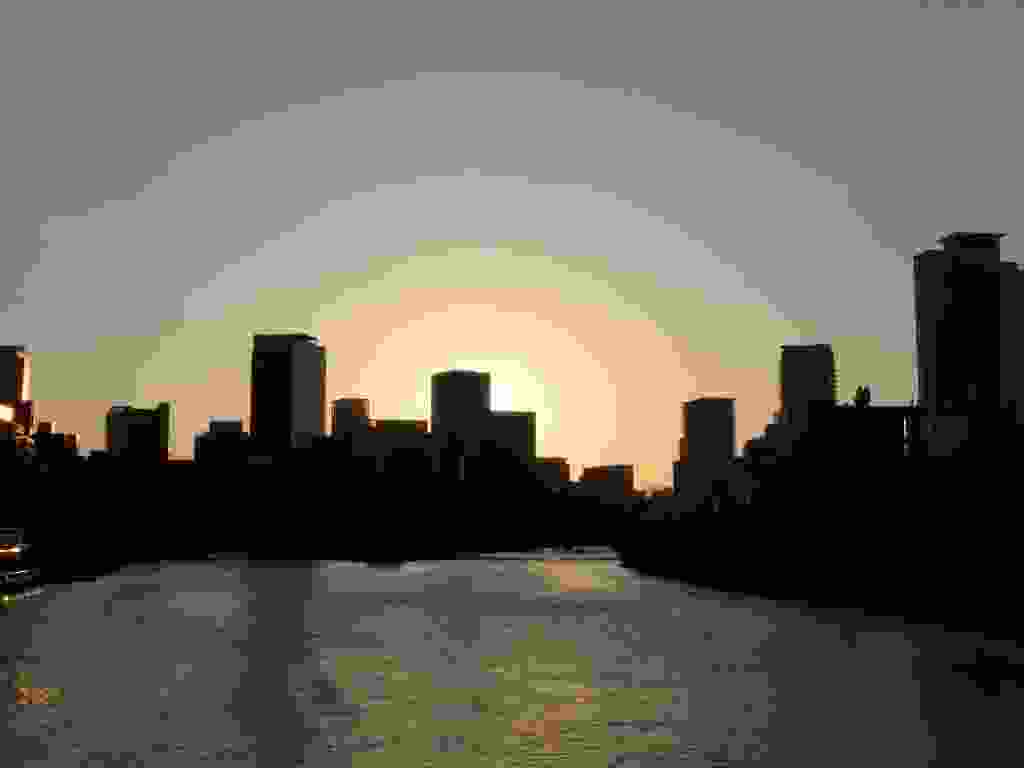
\includegraphics[width=\mywidth]{../wp-content/uploads/2015/09/P8276521-1024x768.jpg} } 
 \newline
 Rue commerçante Tenjimbashisuji, la plus longue du Japon : plus de 2km \newline
 \newline
\centerline{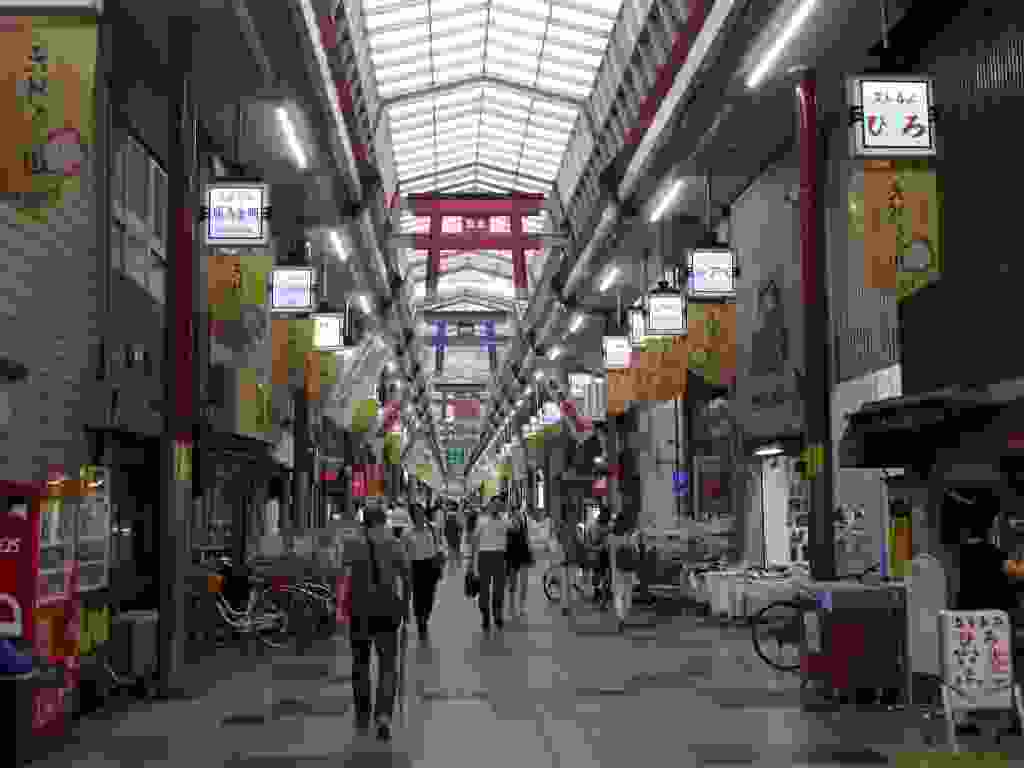
\includegraphics[width=\mywidth]{../wp-content/uploads/2015/09/P8256485-1024x768.jpg} } 
 \newline
 Immenses enseignes le long de la rivière Dotonbori \newline
 \newline
\centerline{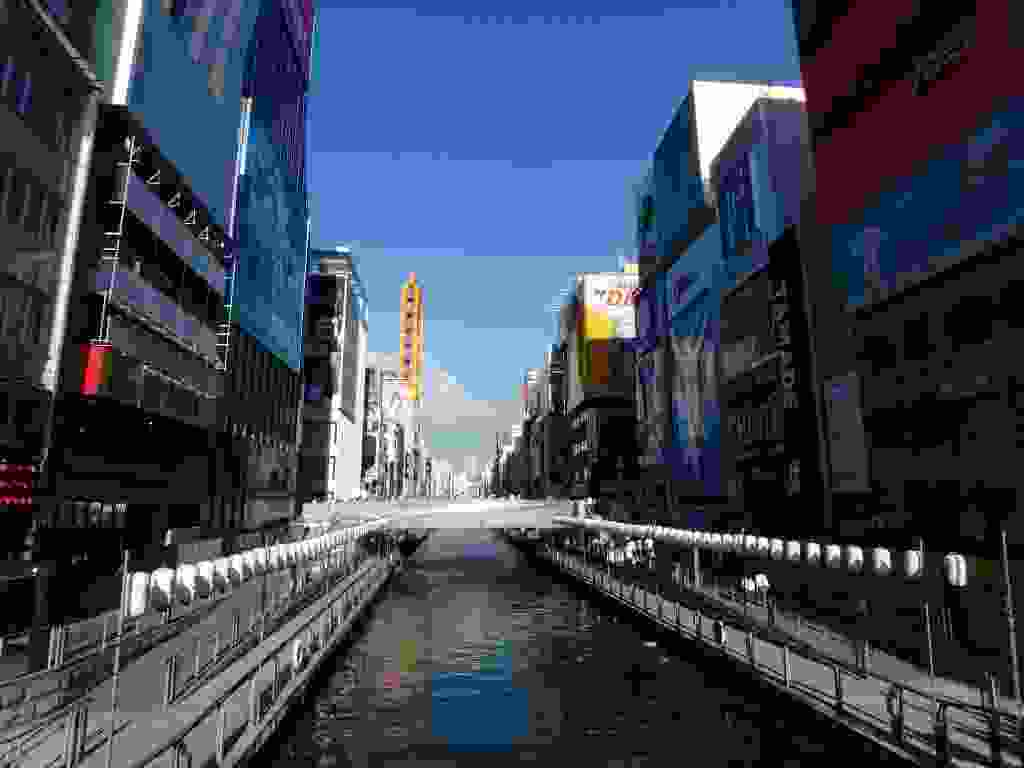
\includegraphics[width=\mywidth]{../wp-content/uploads/2015/08/P8276502-1024x768.jpg} } 
 \newline
 \newline
\centerline{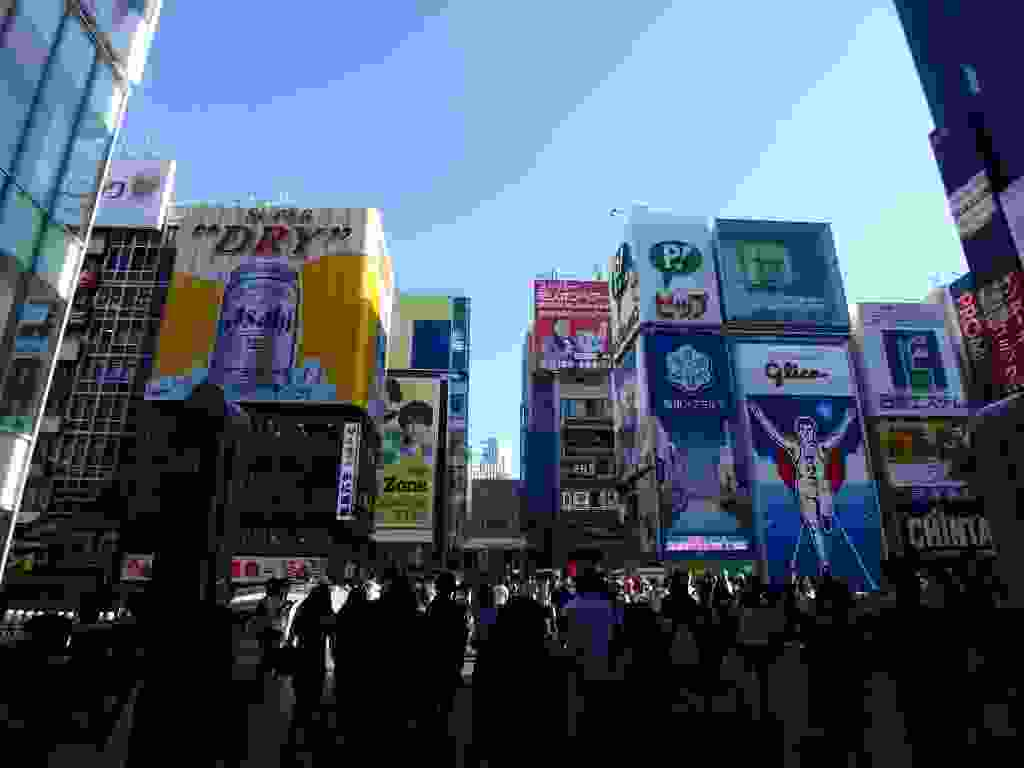
\includegraphics[width=\mywidth]{../wp-content/uploads/2015/08/P8276506-1024x768.jpg} } 
 \newline
 \newline
\centerline{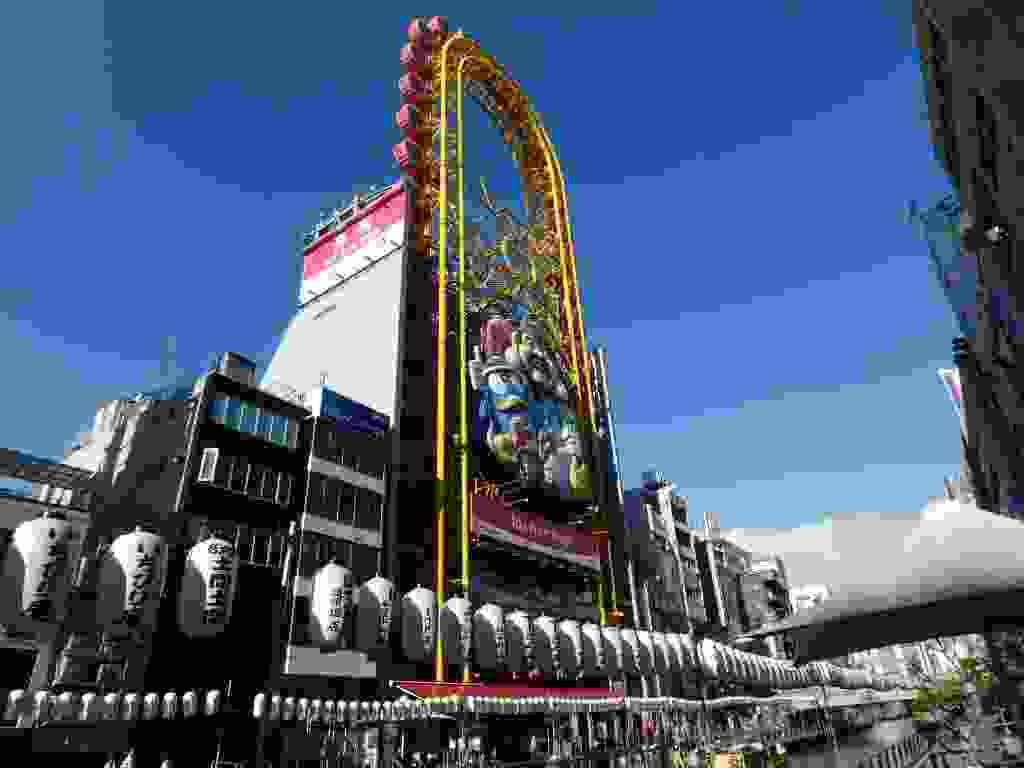
\includegraphics[width=\mywidth]{../wp-content/uploads/2015/09/P8276503-1024x768.jpg} } 
 \newline
 Quartier Tennoji et la tour Tsutenkaku \newline
 \newline
\centerline{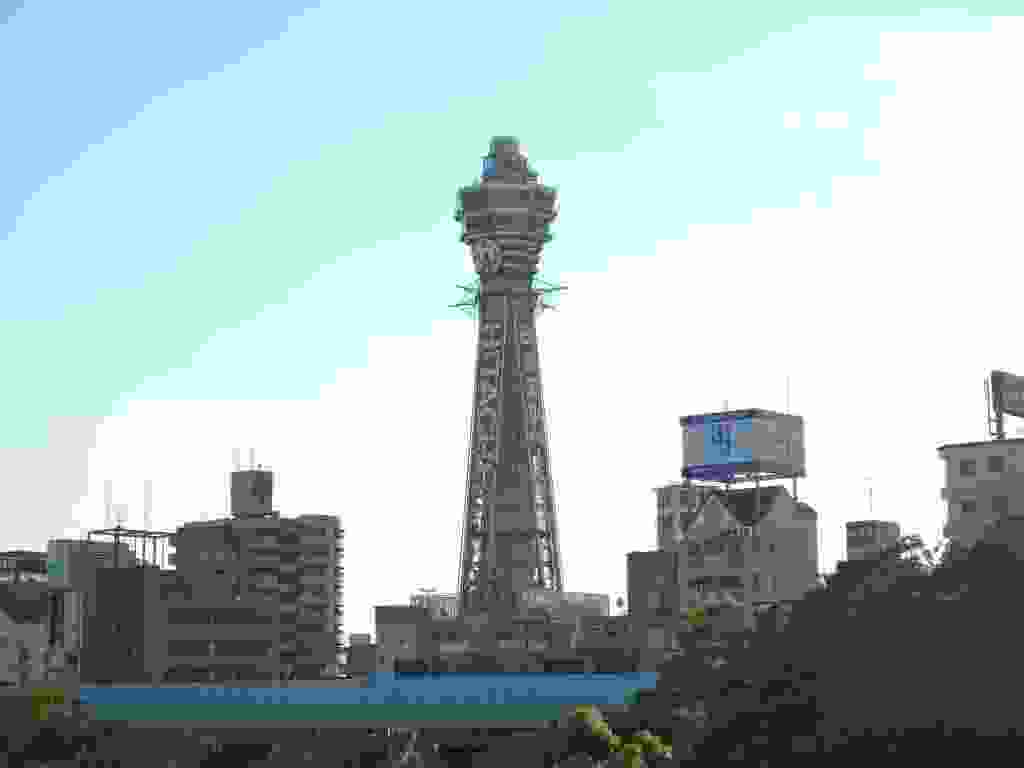
\includegraphics[width=\mywidth]{../wp-content/uploads/2015/08/P8276515-1024x768.jpg} } 
 \newline
 \newline
\centerline{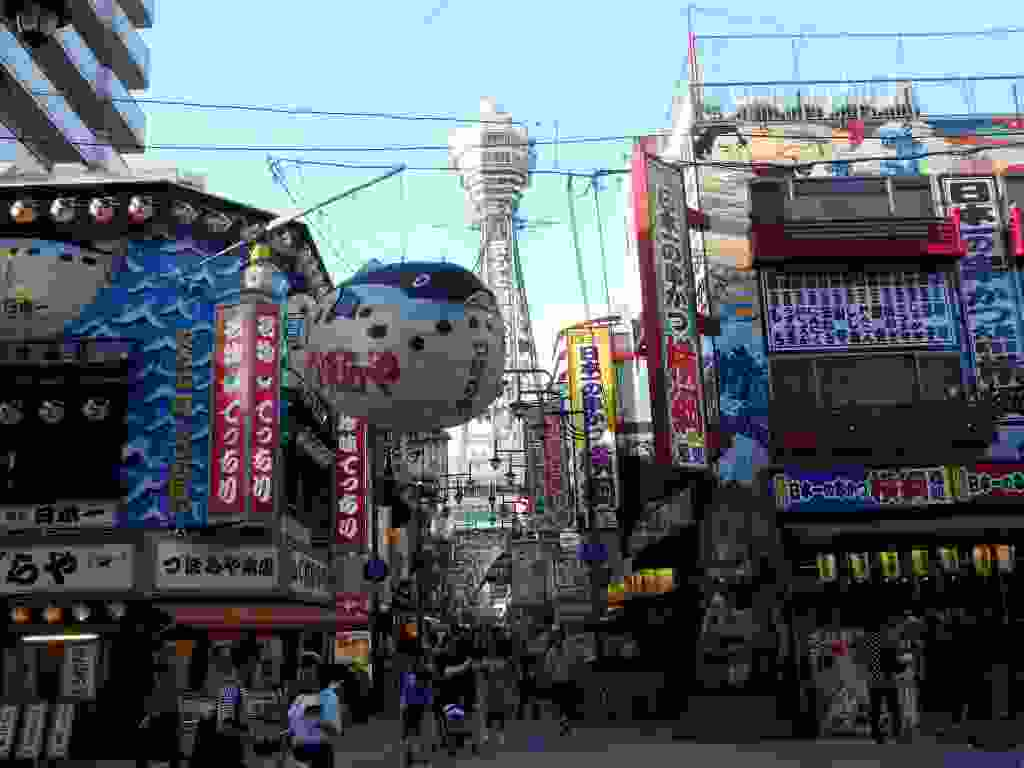
\includegraphics[width=\mywidth]{../wp-content/uploads/2015/08/P8276519-1024x768.jpg} } 
 \newline
 Le building le plus haut du Japon \newline
 \newline
\centerline{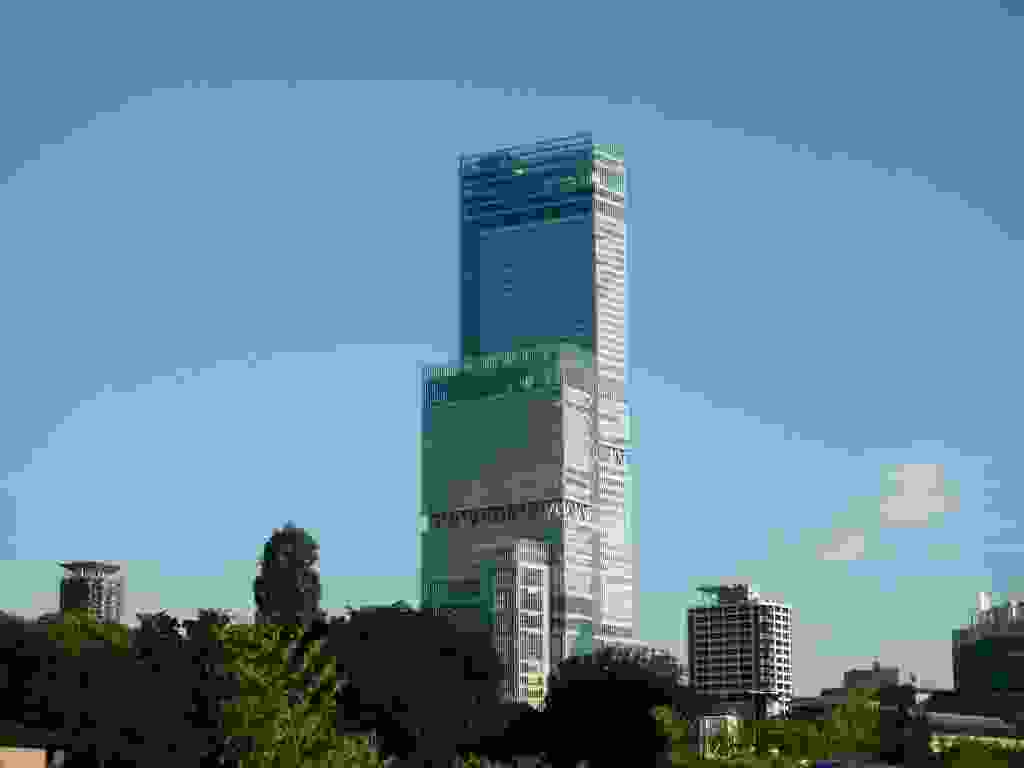
\includegraphics[width=\mywidth]{../wp-content/uploads/2015/09/P8276516-1024x768.jpg} } 
 \newline
 Le temple Shitennoji construit il y a environ 1400 ans \newline
 \newline
\centerline{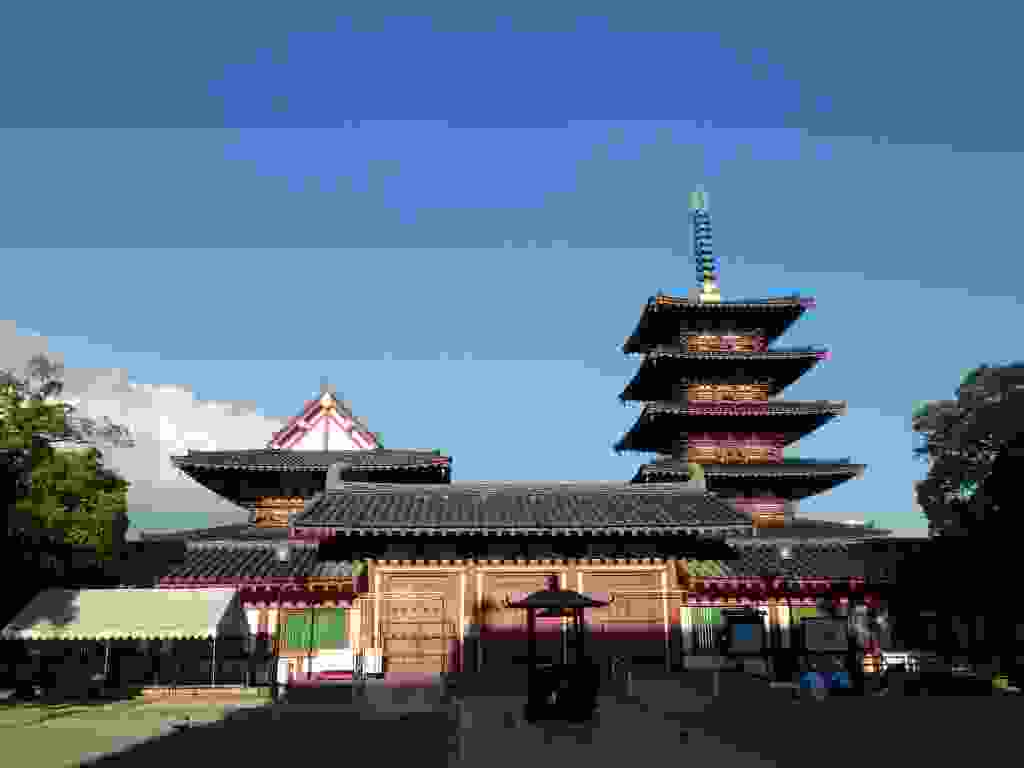
\includegraphics[width=\mywidth]{../wp-content/uploads/2015/09/P8276510-1024x768.jpg} } 
 \newline
 Enfin le château d'Osaka qui a été reconstruit récemment au milieu d'un beau parc \newline
 \newline
\centerline{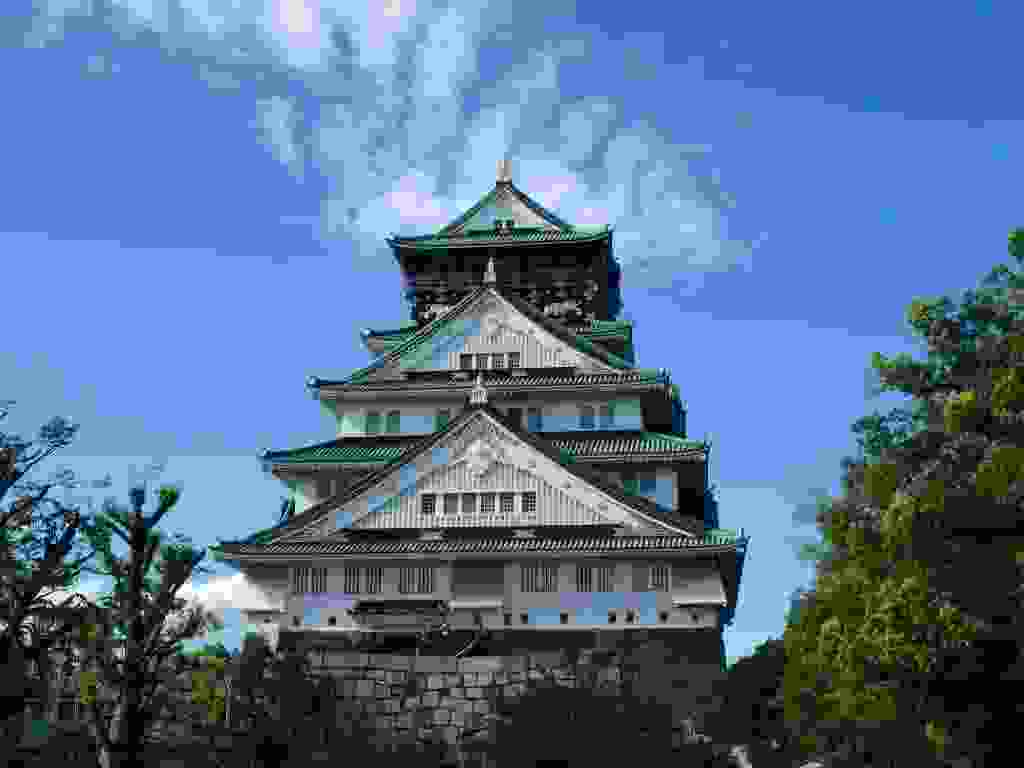
\includegraphics[width=\mywidth]{../wp-content/uploads/2015/08/P8266497-1024x768.jpg} } 
 \newline
 \newline
\centerline{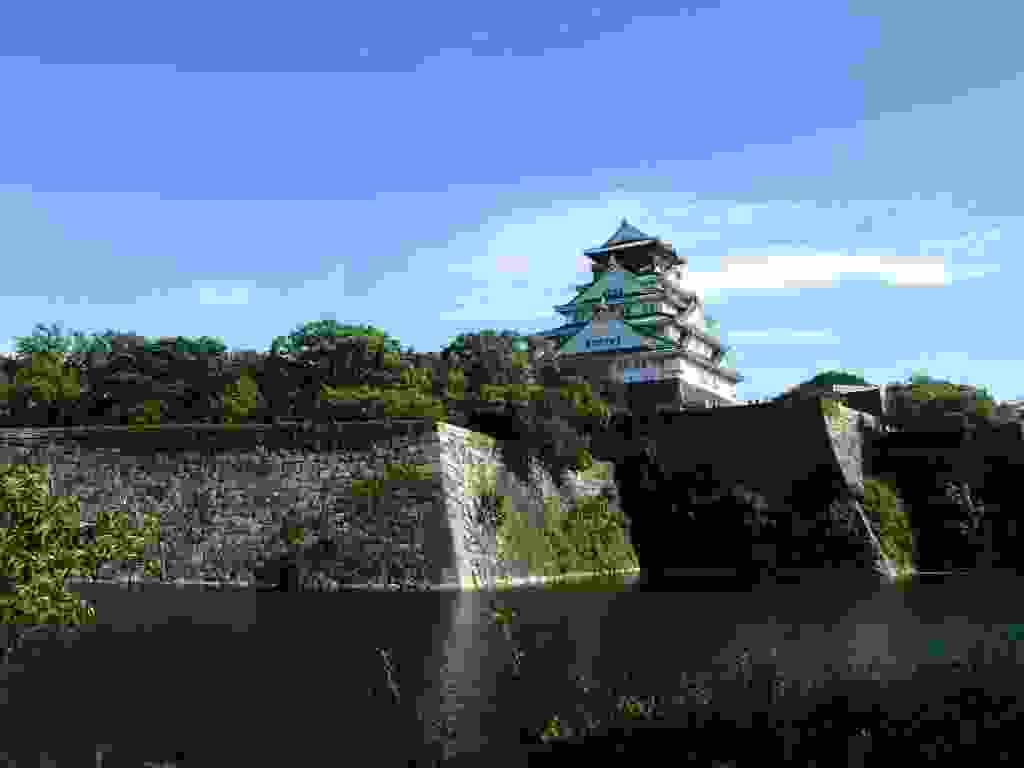
\includegraphics[width=\mywidth]{../wp-content/uploads/2015/09/P8266501-1024x768.jpg} } 
 \newline
 Les salles de Pachinko, il y en a partout dans les villes, le bruit à l'intérieur est incroyable. \newline
 \newline
\centerline{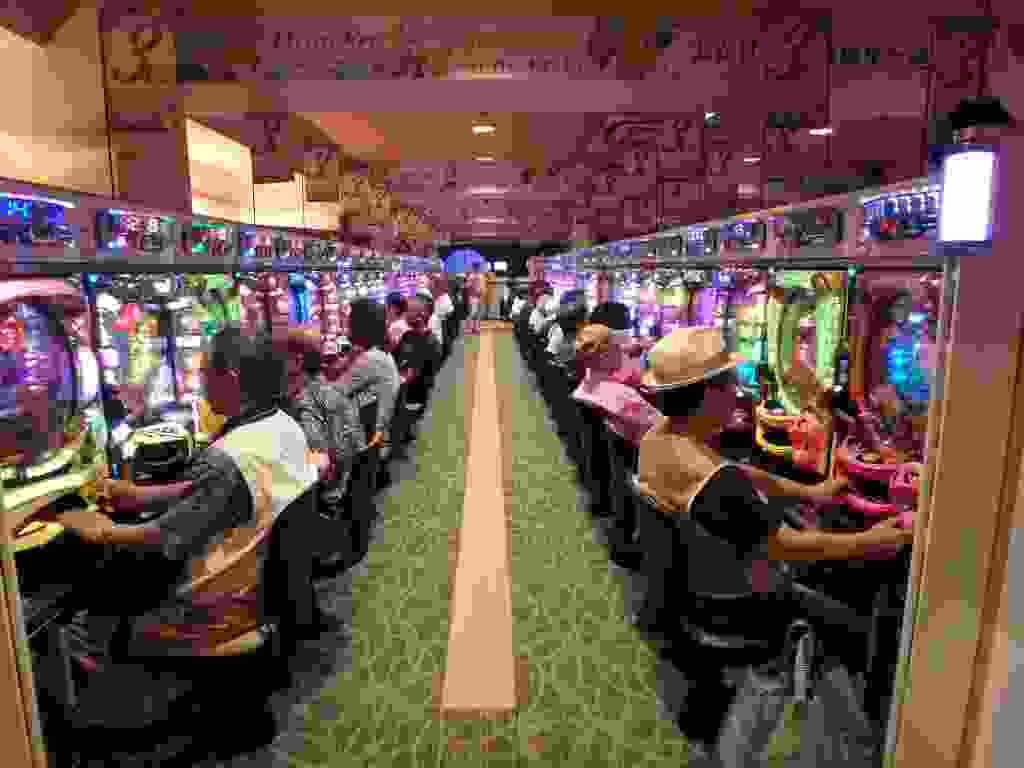
\includegraphics[width=\mywidth]{../wp-content/uploads/2015/08/P8236432-1024x768.jpg} } 
 \newline
 Le golf est populaire au Japon \newline
 \newline
\centerline{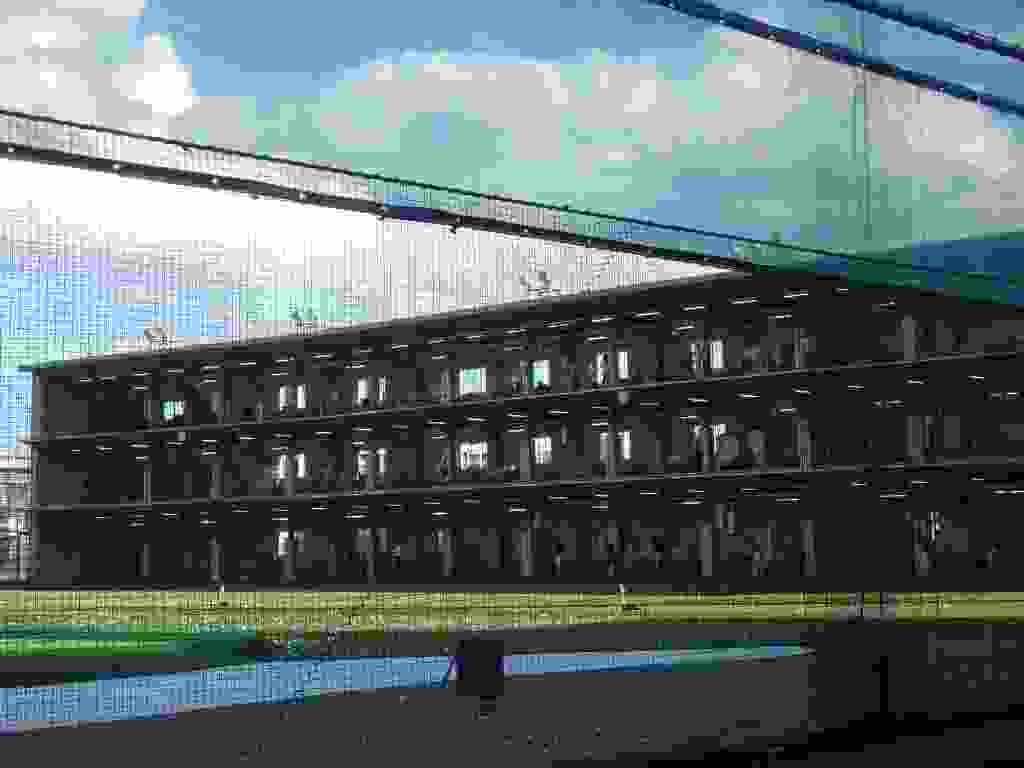
\includegraphics[width=\mywidth]{../wp-content/uploads/2015/09/P8226415-1024x768.jpg} } 
 \newline
 Le tempura, légumes frits souvent en accompagnement des soba noodles, nouilles a la farine de sarrasin. \newline
 \newline
\centerline{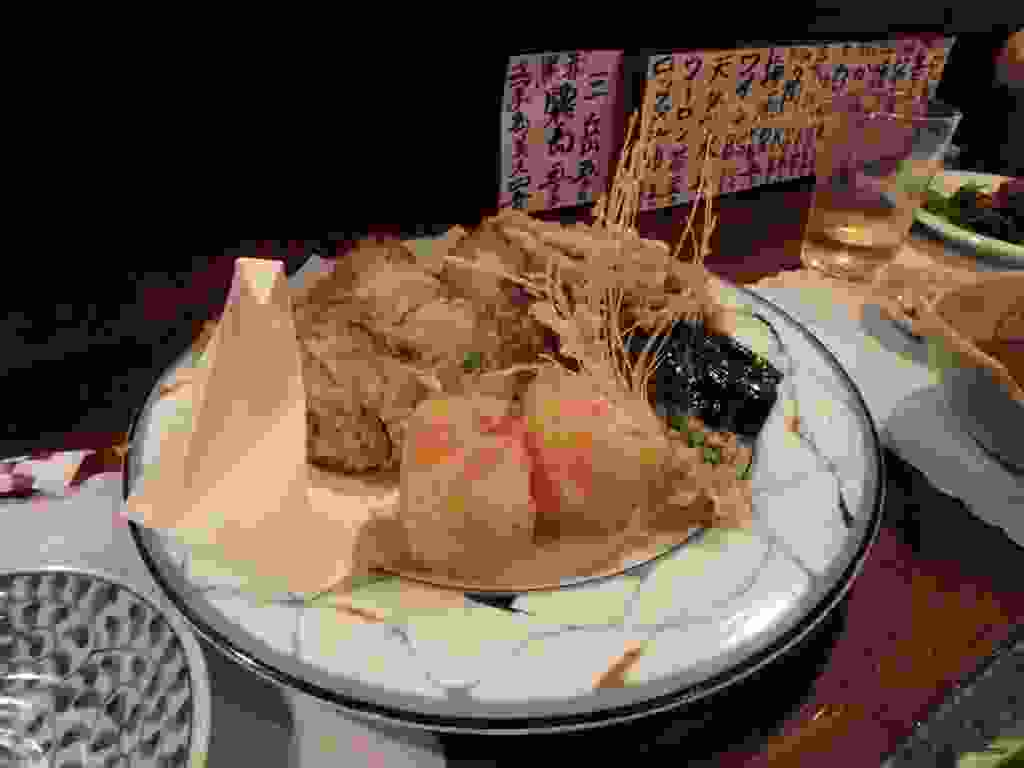
\includegraphics[width=\mywidth]{../wp-content/uploads/2015/08/P8256487-1024x768.jpg} } 
 \newline
 J'ai encore été bien accueilli par plusieurs locaux : \newline
 A Kobé chez la mère de Yukiko qui m'avait hébergée a Tokyo \newline
 \newline
\centerline{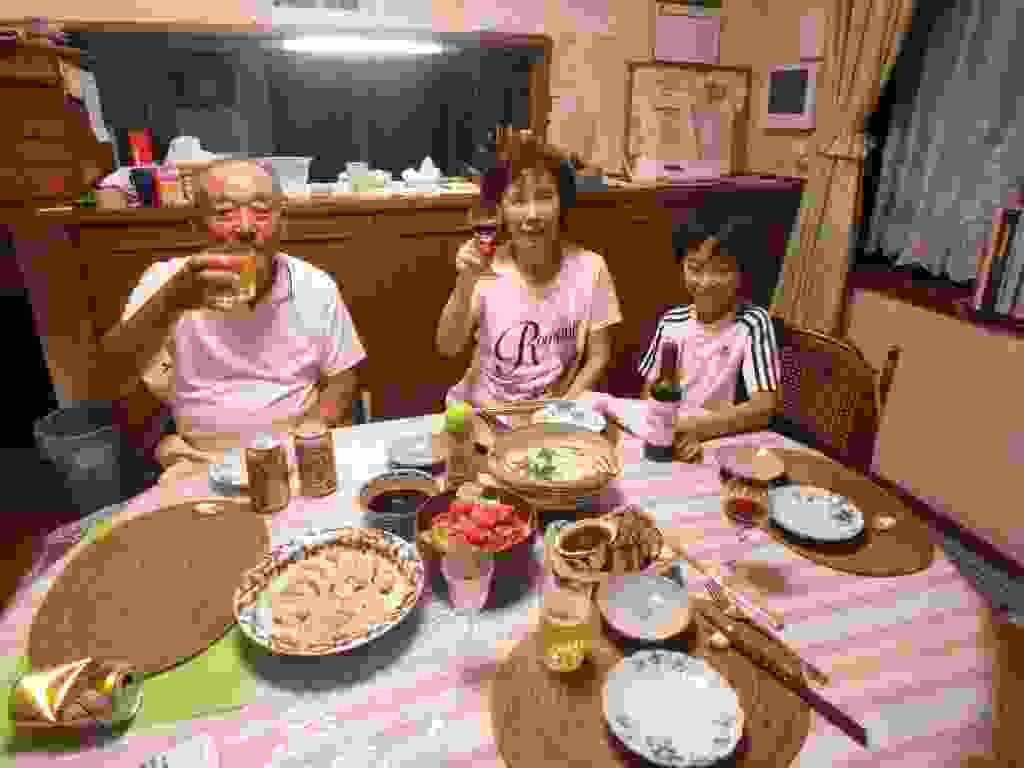
\includegraphics[width=\mywidth]{../wp-content/uploads/2015/08/P8226418-1024x768.jpg} } 
 \newline
 Puis à Osaka chez Fumie qui hébergeait aussi 3 toulousains ! \newline
 Dernière soirée au Japon chez la famille de Emi et Koji qui m'ont preparé un très bon Okonomiyaki \newline
 \newline
\centerline{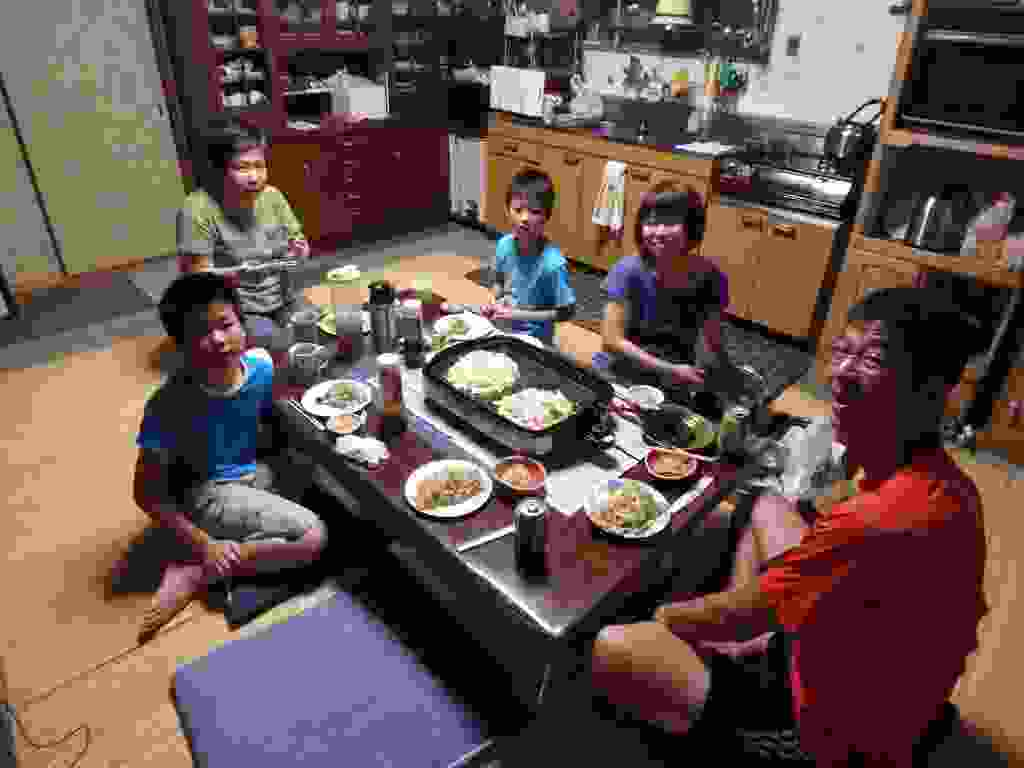
\includegraphics[width=\mywidth]{../wp-content/uploads/2015/08/P8296525-1024x768.jpg} } 
 \newline

\newpage
 
